\chapter{Multi-scale modelling of dry granular flows}

\ifpdf
    \graphicspath{{Chapter4/figs/raster/}{Chapter4/figs/pdf/}{Chapter4/figs/}}
\else
    \graphicspath{{Chapter4/figs/vector/}{Chapter4/figs/}}
\fi

\section{Introduction}

In nature, instabilities of slopes or cliffs are dramatic events involving 
sudden release of a large mass of soil. However, the prediction of catastrophic 
events still represents  challenge, one difficulty being our incomplete 
understanding of the dynamics of granular flows~\citep{Rondon2011}.  
Understanding the mechanics is of particular importance for risks assessment. 
Small scale laboratory experiments are usually unable to properly capture the 
dynamics of geophysical events. However, they can be useful to precisely study 
physical mechanisms, which may play a role in real flows~\citep{Iverson1997}. 

Conventionally, granular materials such as soils are modelled as a continuum. 
On a macroscopic scale, granular materials exhibit many collective phenomena 
and the use of continuum mechanics to describe the macroscopic behaviour can be 
justified. However, on a grain scale, the granular materials exhibit complex 
solid-like and/or fluid-like behaviour depending on how the grains interact 
with each other. Numerical studies at grain scale allows a precise 
understanding of the internal flow structure. Recent works on granular 
materials suggest that a continuum law may be incapable of revealing 
in-homogeneities at the grain-scale level, such as orientation of force chains, 
which are purely due to micro-structural effects~\cite{Rycroft2009a}. Discrete 
Element approaches are capable of simulating the granular material as a 
discontinuous system allowing one to probe into local variables such as 
position, velocities, contact forces, etc. The fundamental question is how to 
model granular materials which exhibit complex phenomenon. It is important to 
understand the mechanics of granular flows and the ability and limitations of 
continuum methods in capturing the flow dynamics.


\section{Granular column collapse}

The collapse of a granular column, which mimics the
collapse of a cliff, has been extensively studied in the case of
dry granular 
material~\citep{Lube2005,Lajeunesse2004,Kerswell2005,Zenit2005,Staron2007a,Hogg2007,Lo2009}.
The granular column collapse experiment involves filling a rectangular channel 
of height $H_0$ and width $L_0$ with a granular material of mass 
`m' (see~\cref{fig:exp}). The granular column is then released \textit{en 
masse} by quickly removing the gate, thus allowing the granular material to 
collapse onto the horizontal surface, forming a deposit having a final height 
$H_f$ and length $L_f$. Despite the complexity of the intermediate flow 
dynamics, experimental investigations have shown that the flow evolution, the 
spreading velocity, the final extent of the deposit, and the energy dissipation 
can be scaled in a quantitative way independent of the substrate properties, 
grain size, density, and shape of the granular material and released 
mass~\citep{Staron2007a,Lajeunesse2005,Lube2005}. The granular collapse has 
also been studied using discrete element method, which allows precise 
measurement of the internal flow 
structure~\citep{Lo2009,Staron2006a,Staron2007a,Utili2014}.
Power laws relating the final run-out and height to the initial aspect ratio of 
the column were observed. These findings immediately pose the question: are 
these simple scaling fortuitous, an oversimplification, or in fact indicative 
of a simple dynamical balance? 


Granular flows are conventionally modelled as a frictional dissipation process 
in continuum mechanics but the lack of influence of inter-particle friction on 
the energy dissipation and spreading dynamics~\citep{Lube2005} is surprising. 
However,~\citet{Kerswell2005} showed the run-out behaviour has a clear material 
dependence, which corroborates the conclusion of~\citet{Lajeunesse2004} and 
softens that of~\citet{Lube2005}. The collapse of a granular column on a 
horizontal surface is a simple case of granular flow, however a proper model 
that describes the flow dynamics is still lacking. Simple mathematical models 
based on conservation of horizontal momentum capture the scaling laws of the 
final deposit, but fail to describe the initial transition regime. From a 
theoretical point of view, the spreading has been described using depth 
averaged equations~\citep{Kerswell2005,Larrieu2006}. The depth-averaged and 
Saint-Venant equations struggle to recover the precise dynamic behaviour of the 
system~\citep{Warnett2013} and only succeeds in predicting the scaling observed 
for aspect ratio less than one. However, describing larger aspect ratio and 
capturing the initial stage of the collapse, when the grains experience a rapid 
change of direction from vertical to horizontal, remain an open challenge, 


\begin{figure}[tbhp]
\centering
\includegraphics[width=0.85\textwidth]{experiment_setup}
\caption{Schematic of experimental configuration for 2-D collapse in a 
rectangular channel,~\citep{Lajeunesse2004}}
\label{fig:exp}
\end{figure}

In the present study, multi-scale numerical modelling, i.e. grain-scale 
modelling and continuum analyses, of the quasi-two dimensional collapse of 
granular columns are performed using Discrete Element (DEM) approach and 
Generalised Interpolation Material Point Method (GIMPM). GIMPM, a hybrid 
Eulerian -- Lagrangian approach, with Mohr-Coloumb failure criterion is used to 
describe the continuum behaviour of granular column collapse. While the 
micro-mechanics of the flow is captured using DEM simulations. Comparing the 
grain scale behaviour with the continuum simulations highlights the limitations 
of continuum approaches in modelling the dense granular flows and their ability 
(or lack thereof) in capturing the complex micro-scale rheology.

\subsection{Numerical set-up}

In this study, numerical simulations of granular columns are analogous to the  
experimental investigation of column collapse performed
by~\citet{Lajeunesse2004}. The experimental configuration 
of~\citet{Lajeunesse2004} is shown in \cref{fig:exp}. Granular material of mass 
`\textit{M}' was poured into a container to form a rectangular heap of length 
`${L}_{\textit{0}}$', height `${H}_{\textit{0}}$' and thickness `\textit{W}'. 
The internal friction angle and the wall friction between the wall and the 
glass beads measured by ~\citet{Lajeunesse2004} are listed 
in~\cref{table:mat_prop}. The gate was then quickly removed to 
release the granular mass that spreads in the horizontal channel until it comes 
to rest. The final run-out distance `${L}_{\textit{f}}$' and the collapsed 
height `$H_{\textit{f}}$' were measured. The run-out distance and collapse 
height exhibit a power law relation with the initial aspect ratio 
`\textit{a}' $(=H_{\textit{0}}/L_{\textit{0}})$ of the column. 

\begin{table}[tbhp]
\caption{Material properties of glass ballotini~\citep{Lajeunesse2004}}
\label{table:mat_prop}
\centering
\begin{tabular}{ll}
\toprule
\textbf{Parameter} & \textbf{Value} \\ \midrule
Mean diameter & 1.15 \si{\mm} \\
Repose angle & 22$\pm 0.5$\si{\degree} \\
Avalanche angle & 27.4$\pm 0.5$\si{\degree} \\
Wall friction angle & 24.8$\pm 0.2$\si{\degree}\\
\bottomrule
\end{tabular}
\end{table}


Granular materials when released suddenly on a 
horizontal surface exhibit transient flow. In this study, the mechanism of flow 
initiation, spreading dynamics and energy dissipation are studied for varying 
initial aspect ratios of the granular column. DEM soil grain characteristics 
match that of the experiment. The particle size distribution (PSD) is one of 
the most important factors controlling landslide initiation and soil 
permeability. Cumulative $\beta$ distribution (described 
in~\cref{sec:beta_dist}) %TODO: Add section reference
 is used to generate a graded sample with a mean grain diameter of 1.15\si{\mm} 
 (see~\cref{fig:PSD}). 
The DEM sample is composed of $\sim3000$ disks with a uniform distribution of 
diameters by volume fractions in the range $[d_{min}, d_{max}] = 0.92 -- 1.38$ 
\si{\mm} with polydispersity $r = \frac{d_{max} }{d_{min}} = 1.5$. The 
granular column is prepared by allowing the randomly placed grains to undergo 
ballistic deposition with a constant potential head between layers of soil 
grains. A snapshot of the sample generated is shown in~\cref{fig:a4b4r18}. A 
DEM sample with soil grains arranged in a regular hexagonal lattice is also 
used to study the influence of crystallisation and jamming on the run-out 
behaviour.
%TODO: Add section reference for sample generation. 

\begin{figure}[tbhp]
\centering
\begin{subfigure}[b]{0.95\textwidth}
\centering
\includegraphics[width=0.5\textwidth]{a4b4r18}
\caption{DEM sample prepared using ballistic deposition}
\label{fig:a4b4r18}
\end{subfigure}
\\
\begin{subfigure}[b]{0.95\textwidth}
\centering
\includegraphics[width=\textwidth]{PSD}
\caption{DEM grains generated using the cumulative $\beta$ distribution}
\label{fig:PSD}
\end{subfigure}
\caption{DEM sample characteristics}
\label{fig:DEM_Sample}
\end{figure}


The overlap between grains are determined by the stiffness 
$\textit{k}_{\textit{n}}$ of the spring in the normal direction. Typically, 
an average overlap in the range 0.1 to 1.0\% is desirable~\cite{Zenit2005} and 
the spring constant is chosen to produce grain overlaps in this range. The 
stiffness is determined as
\begin{align}
& \textit{k}_{\textit{n}}=\frac{2 \pi G}{(1-\nu)[2\ln(\frac{2r}{A})-1]} \\ 
& A = [\frac{2r(1-\nu)f_{n}}{\pi G}]^{\frac{1	}{2}}\,,
\end{align}
where $f_{n}$ is the normal contact force; G is the shear modulus; $\nu$ is the 
Poisson's ratio and r is the radius of the grain. A simpler form of stiffness 
for a spherical grain is defined as
\begin{equation}
\textit{k}_{\textit{n}}=4ER\,,
\end{equation}
where E is the Young's modulus of the material and R is the radius of the 
grain.~\citet{Cambou2009} observed that the contact model has negligible 
influence on the run-out behaviour of rapid granular flows. The granular 
collapse simulations performed using non-linear Hertz-Mindlin contact model and 
the linear-elastic contact model showed no significant difference on the 
granular flow behaviour~\citet{Utili2014}. Linear-elastic contact model is used 
in the present study due to its simplicity and lower computation time 
requirement. The maximum tangential force is limited by the Mohr-Coloumb 
criterion. 


\citet{Staron2006a} observed that the coefficient of restitution $\varepsilon$ 
was dramatically changing the behaviour of the systems for 
$\varepsilon\longrightarrow 1$; in particular, this dramatic change is expected 
to become more important for increasing values of a. On the contrary, for 
$\varepsilon \le 0.8$, the influence of the coefficient of restitution becomes 
negligible. In the present study, a value of 0.75 is adopted as the coefficient 
of restitution, similar values of restitution coefficient was adopted 
by~\citet{Zenit2005,Girolami}. The normal damping coefficient 
$C_{\textit{n}}$ 
is appropriately chosen to achieve the required coefficient of restitution 
$\varepsilon$:
\begin{align}
& C_{\textit{n}}=2\gamma \sqrt{m_{\textit{ij}}k_{\textit{n}}} \\ 
& \mbox{where} \quad \gamma = -\frac{\ln(\varepsilon)}{\sqrt{\pi^{2}+\ln^2 
(\varepsilon)}},\quad \mbox{and} \quad 
\textit{m}_{\textit{ij}}=\frac{\textit{m}_{\textit{i}}\textit{m}_{\textit{j}}}{\textit{m}_{\textit{i}}
 + \textit{m}_{\textit{j}}} \,.
\end{align}
%
The micro-mechanical parameters used in this study are presented 
in~\cref{table:DEM_data}. Due to the unsteady nature of the flow, the 
grains get dispersed on the horizontal plane as discrete bodies start to 
separate from the main mass, hence the run-out distance is calculated as the 
position of the farthest grain which has at least one contact with the main 
mass.

\begin{table}
\caption{Micro-mechanical parameters used in DEM simulations}
\label{table:DEM_data}
\centering
\begin{tabular}{ll}
\toprule
\textbf{Parameter} & \textbf{Value} \\ \midrule
Young's modulus of glass bead & $70\times10^{9}$ \si{\newton\per\m\squared}\\ 
Poisson's ratio & 0.22 - 0.24\\ 
Diameter of glass beads & 0.92 to 1.38 \si{\mm}\\
Normal and shear stiffness of grains & $1.6 \times 10^{8}$ \si{\newton\per\m}\\ 
Normal and sear stiffness of wall & $4 \times 10^{8}$ \si{\newton\per\m}\\
Inter-particle friction coefficient, $\mu$ & 0.53 \\
Wall friction coefficient & 0.466 \\ 
Coefficient of restitution, $\varepsilon$ & 0.755 \\ \bottomrule
\end{tabular}
\end{table}

GIMPM with Mohr-Coloumb constitutive model is used to simulate plane strain 
collapse of granular columns.~\citet{Crosta2009} observed that the Mohr-Coloumb 
with non-associate flow rule is able to capture granular collapse dynamics and 
models the strong vertical motion components, but it does not suffer the 
limitations of typical shallow water equation methods. In order to understand 
the ability and limitations of continuum approaches in capturing the local 
rheology, it is important to scale the grain scale properties, such as 
inter-particle friction and stiffness, to the continuum 
scale (macroscopic friction and Young's modulus).~\citet{Crosta2009} observed 
that the friction angle plays a significant role on the run-out behaviour. In 
MPM simulations, the granular flow is assumed to be in critical state and the 
critical state friction angle is used in the Mohr-Coloumb model. In order to 
obtain the critical state friction angle of the granular sample, a shear test 
is performed using 1078 DEM grains. A bi-periodic boundary condition is adopted 
on the sides of the sample (see~\cref{fig:shear}. Two layers of fixed grains 
(shown in black) is placed at the top and the bottom of the shear sample. A 
normal pressure `P' and a horizontal velocity \textit{v} is applied to the 
fixed grains  at the top of 
the shear sample. The normal effective stress is varied in the sample and the 
average shear stress of the sample is measured. The sample was sheared until 
critical state was reached. The slope of shear stress 
versus normal effective stress gives the critical state friction angle. A 
critical state friction angle of $22.2$\si{\degree} is obtained. The 
macroscopic friction angle is in the range observed 
by~\citet{Estrada2008,Mitchell2005}. The Young's 
modulus of the granular assembly is obtained as the initial slope of the 
stress-strain plot of a uni-axial compression of a granular column using DEM.

\begin{figure}
\centering
\begin{subfigure}[b]{0.4\textwidth}
\centering
\includegraphics[width=\textwidth]{simple_shear}
\caption{Boundary conditions}
\label{fig:shear}
\end{subfigure}
\begin{subfigure}[b]{0.575\textwidth}
\centering
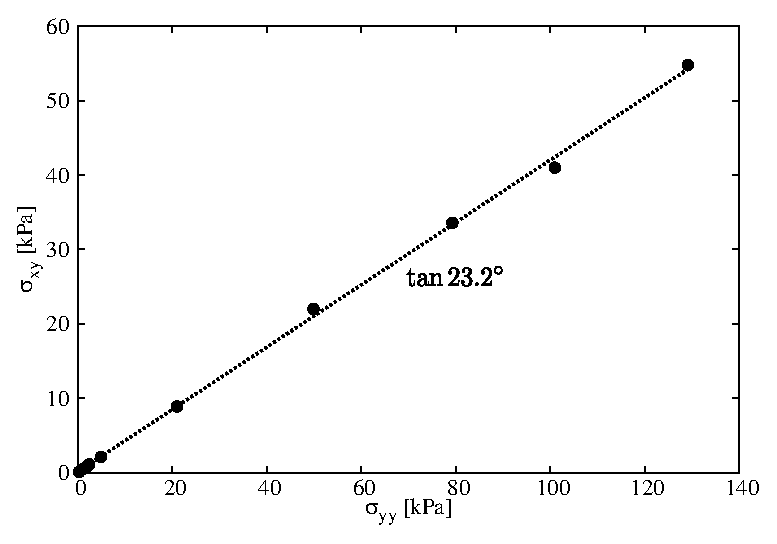
\includegraphics[width=\textwidth]{Sxy_vs_Syy}
\caption{Critical state friction angle from periodic shear test}
\label{fig:Sxy_vs_Syy}
\end{subfigure} 
\caption{Periodic shear test}
\label{fig:shear_test}
\end{figure}

\citet{Guilkey2003} suggests using at least four material points per cell for 
large deformation problems. In the present study, 16 material points 
per cell is adopted. If the mesh is too fine and the number of particles is too 
large, the particle size $2lp$ decreases, and the GIMPM interpolation 
function 
tends to approach the original MPM function, as shown 
by~\citet{Bardenhagen2004}. Hence GIMPM loses the merit that it reduces the 
numerical noise due to material points crossing the background mesh. In 
addition, the probability of particles crossing the background mesh increases 
with decrease in mesh size, hence, more noise can be produced~\cite{Abe2013}. 
The effect of number of material points per cell on the run-out behaviour is 
discussed in~\cref{sec:MPM_points_per_cell}. Each material point represents 
one-fourth of a DEM soil grain. The parameters used for the continuum analyses 
are presented in~\cref{table:MPMData}. 

\begin{table}
\caption{Parameters used in continuum simulations}
\label{table:MPMData}
\centering
\begin{tabular}{ll}
\toprule
\textbf{Parameter} & \textbf{Value} \\ \midrule
Material point spacing & 0.575 \si{\mm} \\
Number of material points per cell & 16 \\
Young's Modulus, E & $1.98 \times 10 ^{6}$ \si{\Pa} \\
Poisson's ratio, $\nu$ & 0.22 to 0.24 \\ 
Friction angle, $\phi$ & $23.2 \pm 0.2\si{\degree}$ \\
Dilatancy angle, $\varPhi$ & $0$\si{\degree} \\
Density, $\rho$ & 1800 \si{\kg\per\m\cubed}\\
Wall friction & 0.466 \\
Time step increment & $1.0 \times 10^{-6}$ \si{\second}\\ \bottomrule
\end{tabular}
\end{table}

\subsection{Deposit morphology}
MPM and DEM simulations of granular column collapse are 
performed by varying the initial aspect ratio of the column. 
The normalized final run-out distance, $\Delta L = 
(L_{\textit{f}}-L_{\textit{0}})/L_{\textit{0}}$, as a function of the initial 
aspect 
ratio `a' of the column is presented in~\cref{fig:run-out}. Similar to the 
experimental 
behaviour a power law relation between the run-out and the initial aspect ratio 
of the 
column is observed. Two distinct flow regimes can 
be seen: (a) for `a' <1.7 a linear relation between the spread and aspect ratio 
can 
be observed, and (b) for `a' > 1.7 a power-law relationship exists. In the 
present study, 
the following scaling law for the run-out (using DEM) is observed:
\begin{align}
\frac{L_{\textit{f}}-L_{\textit{0}}}{L_{\textit{0}}} \approx  
\begin{cases}
1.67 a, &\qquad \textit{a}\lesssim 2.3 \\
2.5 a^{2/3}, &\qquad \textit{a} \gtrsim 2.3 \\
\end{cases}
\end{align}
Both, MPM and DEM simulations are able to capture the linear relationship for 
`a' < 1.7, 
and the simulation results agree with the experimental 
investigation~\cite{Lajeunesse2005}. This shows that a simple frictional 
dissipation 
model is able to capture the flow dynamics for columns with smaller aspect 
ratio.
For `a' < 1.7, the normalised run-out distance predicted using DEM simulations 
are very 
close to the run-out observed in the experiments. DEM simulations with 
hexagonal 
packing shows shorter run-out distances in comparison to randomly packed 
sample. This difference in the run-out behaviour might be due to the 
crystallisation and 
jamming effects in hexagonal packing. The small difference in the final run-out 
between 
DEM and experimental results can be attributed to the variation in the 
packing of grains. Also, the experimental data corresponds to granular column 
collapse in 
a rectangular channel, the collapse is not a pure two-dimensional collapse as 
in the case 
of numerical simulations. 

Significant difference in the final run-out between MPM, which is based on a 
simple 
frictional model for dissipation of potential energy, and DEM simulations for 
`a' > 1.7 
indicates a change in the mechanism of energy dissipation for columns with 
large aspect 
ratios (`a' > 1.7).~\cite{Staron2005b} observed that a constant frictional 
dissipation 
model cannot describe a power-law relation observed at large aspect ratio. A 
transition 
in the run-out behaviour at an aspect ratio of 1.7 indicates a change in flow 
dynamics. 
Similar behaviour in the run-out distance was observed by~\citet{Bandara2013} 
for columns 
with large the aspect ratio $\ge 2$.

The longer run-out distance in MPM simulations at large aspect ratios might be 
influenced 
by the amount of material mobilised during the collapse. In tall columns, 
the entire column participates in the flow, in contrast to short columns where 
the 
collapse is due to avalanching of flanks,~\citet{Lajeunesse2004}. It is 
possible that 
MPM simulations 
collapses more resulting in longer run-out distance.~\Cref{fig:height} shows 
the normalized final height as a function of the initial aspect ratio of the 
column. 
Similar to the run-out behaviour, the normalised-height also shows two distinct 
regimes. The scaling of final height of the column with the initial 
aspect ratio of the column can be written as
\begin{align}
\frac{H_{\textit{f}}}{L_{\textit{i}}} \propto  
\begin{cases}
\textit{a}, \qquad & \textit{a}\lesssim0.7 \\
\textit{a}^{2/3}, \qquad & \textit{a}\gtrsim0.7 \\
\end{cases}
\end{align} 

The final height predicted by both DEM and MPM simulations match the 
experimental data 
for columns with smaller aspect ratio ($`a' \le 0.7$). Linear relationship 
between the 
final height and the aspect ratio indicates that only a part of the granular 
column is 
mobilised during the collapse. For tall columns, both approaches predict 
similar 
normalised height. However, the normalised height observed in MPM is higher 
than in DEM 
simulations, which is in contrast to the idea of increase in the amount of 
material mobilised during the collapse in MPM simulations resulting in longer 
run-out 
distance. Hence, the longer run-out observed in MPM simulations is due a change 
in the 
flow dynamics at higher aspect ratios, which is not captured in MPM 
simulations. The 
final height of a column is controlled by the amount of static region in the 
granular 
column collapse, while the run-out distance is essentially a function of the 
flowing 
mass. Hence, it is essential to compare the evolution of flow and the internal 
flow 
structure in DEM and MPM simulations.

\begin{figure}[tbhp]
\centering
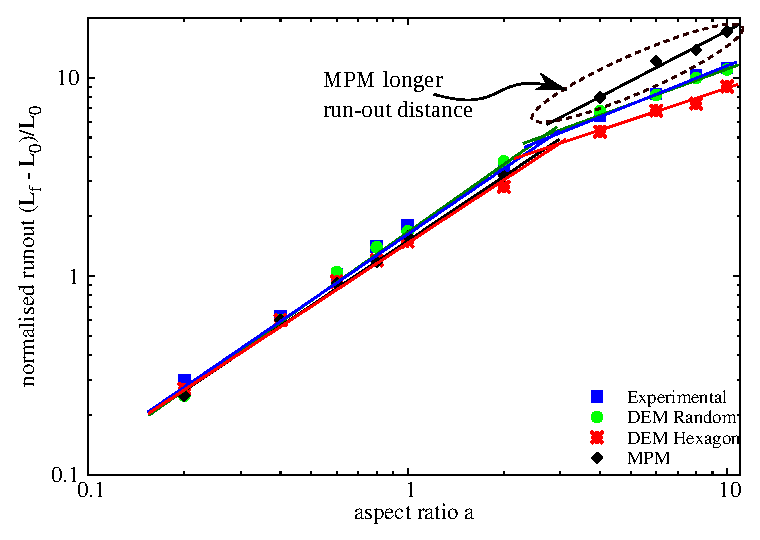
\includegraphics[width=\textwidth]{runout}
\caption{Normalised final run-out distance for columns with different initial 
aspect ratio}
\label{fig:run-out}
\end{figure}

\begin{figure}[tbhp]
\centering
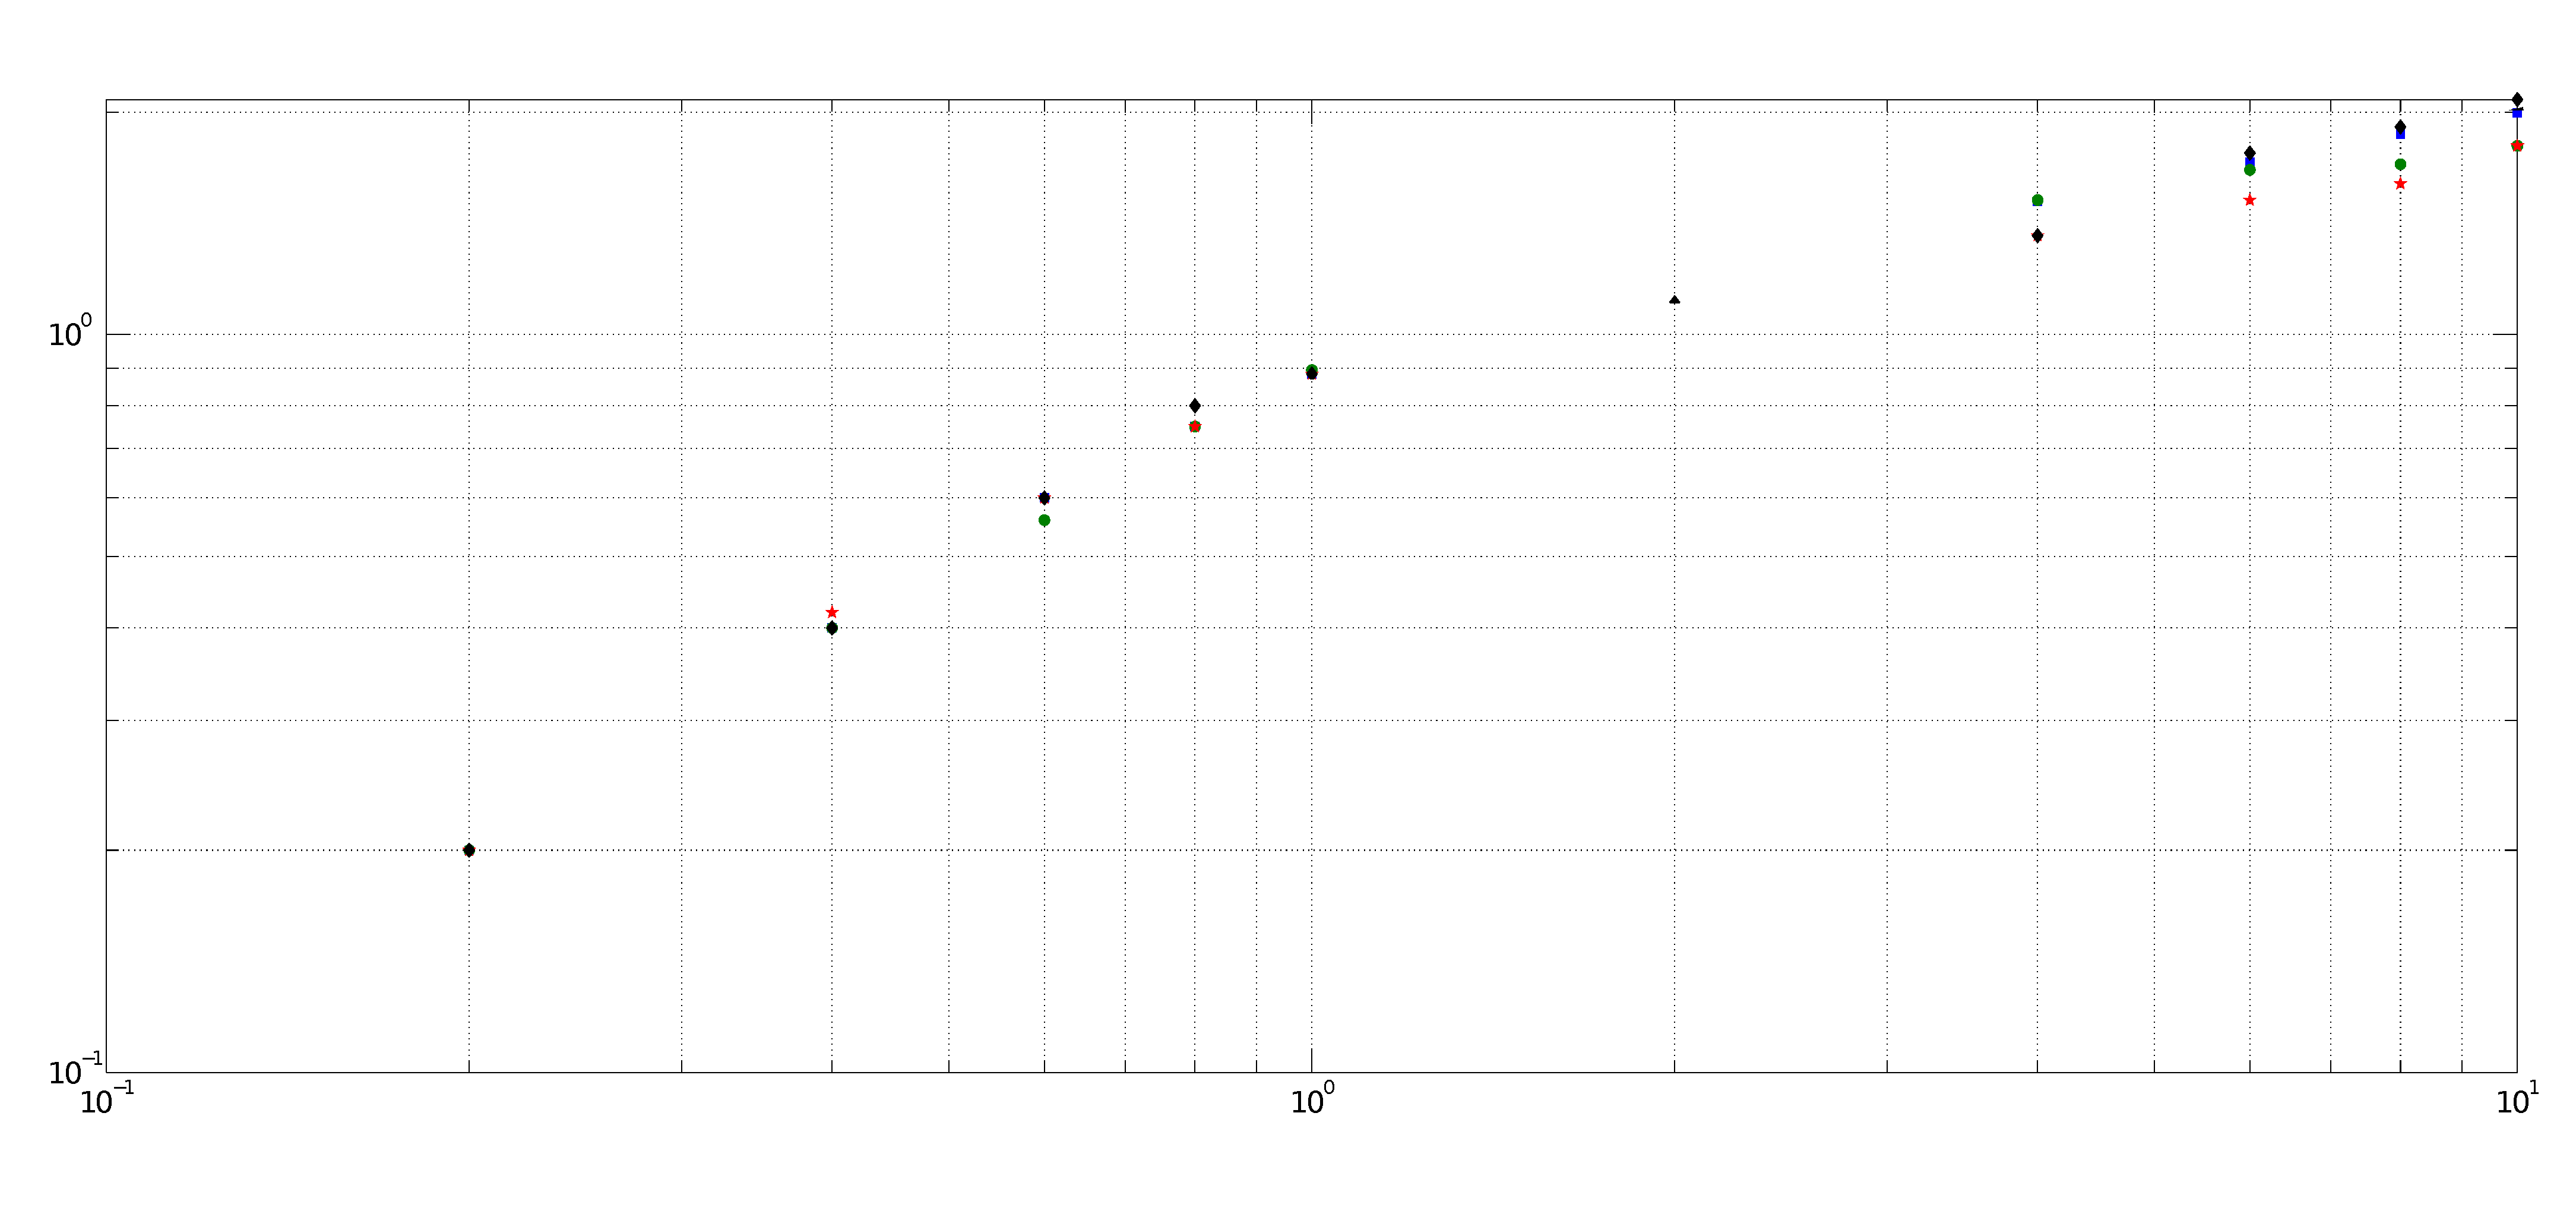
\includegraphics[width=\textwidth]{height}
\caption{Normalised final collapse height for columns with different initial 
aspect ratio}
\label{fig:height}
\end{figure}

\subsection{Flow evolution and internal flow structure}

The normalised run-out and height as a function of the aspect ratio indicates 
that, for a 
given granular material and substrate properties, the flow dynamics 
and the final deposit morphology are independent of the volume of granular 
material 
released, but depend only on the geometry of the column. A 
power law relationship is observed between the run-out distance and the initial 
aspect ratio of the column. A transition in the run-out behaviour at an aspect 
ratio of 2.3 indicates a change in the flow dynamics. 

For smaller aspect columns (`a' < 2.3), the flow is initiated 
by a failure at the edge of the pile along a well-defined fracture surface.
The granular mass fails through avalanching of flanks producing a 
truncated cone-like deposit (`\textit{a}' < 0.7) or conical deposit 
(`\textit{a}' > 0.7). The grains located above the failure surface move 
``\textit{en 
masse}'' leaving a static region underneath the failure surface. 

Dimensional analysis of granular column collapse reveals an intrinsic time 
defined as $\sqrt{H_{\textit{i}}/g}$. This intrinsic time is a transient time 
of order $\tau_{c}$, at which the flow is fully developed, i.e., the potential 
energy available at the initiation of collapse is now fully converted to 
kinetic energy. Numerical simulation of the velocity profile of a granular 
column (`a'=0.4) at critical time $\tau_{c}$ is presented in \cref{fig:a04tc}. 
At critical time, the velocity field depends only on the position of the grain 
along the sliding mass. The maximum velocity is observed at the front of the 
flowing mass corresponding to that of a plug flow in horizontal direction. 
Particulate and continuum simulations show similar run-out distance at the 
critical time. Both approaches show similar quantity of material destabilised 
above the failure surface. However, the crystalline arrangement of soil grains 
in a hexagonal packing results in a different flow mechanics, which also 
shows the effect of jamming at the flow front. The continuum nature of MPM 
results in a slightly different geometry of the material destabilised above the 
failure surface in comparison to DEM simulations. The velocity profile is 
similar to a steady granular surface flow observed by~\citet{Lajeunesse2004}. 

For columns with lower initial aspect ratios, the run-out distance is 
proportional to the mass flowing above the failure surface. The spreading 
results from a Coulomb-like failure of the edges and implies no free fall of 
the column. ~\citet{Daerr1999} also observed active Coulomb yielding in 
transient granular surface flows. In this case, the effective friction 
properties of the flow can be simply predicted from the shape of the final 
deposit. The amount of mass mobilized during the collapse is significantly 
affected by the angle of the failure surface.~\Cref{fig:a04tc} shows that both 
numerical techniques predict a distinct failure surface when the flow is fully 
developed at critical time $\tau_{\textit{c}}$. The angle of the failure 
surface is found to be about $55^{o}$. The failure surface begins from the toe 
of the column and protrudes inwards at an angle of $50$ to 
$55\si{\degree}$. The formation of the ``truncated conical deposit'' or 
``conical deposit'' depends only on the initial length of the column, as the 
angle of the failure surface is found to be independent of the aspect ratio. 
The failure angle is consistent with the interpretation in terms of 
\textit{active Coulomb failure}~\citep{Lajeunesse2004}, which leads to a 
predicted failure angle $\theta_{\textit{y}}=45\si{\degree}+\delta / 2$, where 
$\delta$ is the internal friction angle of the granular material. In the 
present study, the friction angle of the glass beads is $22\si{\degree}$, which 
leads to $\theta_{\textit{y}}=45\si{\degree}+22\si{\degree}/ 2=56\si{\degree}$, 
which is in good agreement with the numerical simulations and experimental 
observations by~\citet{Lajeunesse2004}. The fracture angle has a 
direct effect on the transition between the truncated cone and the conical 
deposit occurring at an aspect ratio of 0.7.~\citet{Schaeffer1990} observed the 
onset of instabilities in a narrow wedges of $56\mbox{ to }65^{o}$ for 
Cambridge-type constitutive models that describes granular flows, which is 
in-line with the failure angle observed in the present study. 

The final profile of the granular column with an initial aspect ratio 
of 0.4 is shown in \cref{fig:a04f}. Both MPM and DEM show similar run-out 
behaviour. The continuum approach is able to capture the flow dynamics of short 
columns, wher the failure mechanism is active Coulomb failure. In dense 
hexagonal packing, the failure surface is steep due to crystallisation effect. 
The variation in the angle of the failure surface causes a difference in the 
amount of material destabilised, and in turn in the run-out distance. 
This crystallisation phenomenon is found to have a significant influence on the 
final deposit of the granular column.~\citet{Lacaze2009} observed that 
poly-disperse grains have lesser tendency to crystallize especially in the case 
of tall columns. 

\begin{figure}[tbhp]
\centering
\includegraphics[width=\textwidth]{a04tc}
\caption{Velocity profile of a granular column collapse ($`a' = 0.4$ \& 
$t=\tau_c$)}
\label{fig:a04tc}
\end{figure}

\begin{figure}[tbhp]
\centering
\includegraphics[width=\textwidth]{a04f}
\caption{Velocity profile of a granular column collapse ($`a' = 0.4$ \& 
$t=3\times\tau_c$)}
\label{fig:a04f}
\end{figure}


For tall columns (`a' > 2.3), the flow is still initiated by a well defined 
failure surface as can be seen in~\cref{fig:a6tc}. However, in this case the 
initial granular column is much higher than the top of the failure surface. Due 
to gravity most of the grains in the column experience free-fall 
consuming the column along their way. When they reach the vicinity of the 
failure surface, the flow gets deviated along the horizontal direction 
releasing a huge amount of kinetic energy gained during the free fall. For 
larger aspect ratio (\textit{a} > 0.7), the resulting static region is a cone, 
the final height of the cone, i.e, $\textit{H}_{\textit{f}}$ lies above the 
summit of the failure surface. Hence, a different evolution is observed from 
that of the axis-symmetric geometry~\citep{Lube2005}, where the final height 
coincides with the summit of the failure surface forming a truncated conical 
deposit.~\citet{Lajeunesse2004} observed that the variation in the deposit 
morphology between the axis-symmetric case and the rectangular collapse to be a 
geometrical effect rather than as an experimental artefact. 

An initial failure surface starting from the toe end 
of the column at an angle of about 55$^{o}$ can be observed at the critical 
time $\tau_{c}$. As the collapse of the granular collapse progresses, 
successive failure planes parallel to the initial failure surface are formed 
and shear failure occurs along these planes. The presence of several shear 
bands in the final profile of the collapsed granular column confirms this 
hypothesis. Crystallisation in hexagonal packing has a significant effect on 
the run-out distance by forming series of parallel shear bands. However, the 
Material Point Method fails to capture the formation of shear bands during the 
collapse. This observation throws light on the mechanics of propagation of 
shear bands in massive landslides such as the Storegga submarine landslide. The 
flow behaviour becomes similar to that of columns with lower aspect ratio as 
the flow starts descending along the failure plane. The final profile 
of the collapsed granular column with an initial aspect ratio of 6 is presented 
in Figure.\ref{fig:a6f}. For tall columns, the dissipation process is more 
complex due to the free-fall dynamics. The vertical acceleration
of the grains induces a non-trivial mass distribution in the flow while 
spreading. This mass distribution plays a dominant role in the power-law 
scaling law obeyed by the run-out~\citep{Staron2006a}.

Regardless of the experimental configuration and the initial aspect ratio of 
the columns, the flow is initiated by a well-defined rupture surface, above 
which the material slides down leaving a static region underneath the failure 
plane. Depending on the aspect ratio of the column, two asymptotic behaviours 
are observed. For smaller aspect ratios, the flow is dominated by friction 
where as large aspect ratio columns are influenced by the pressure gradient.

\begin{figure}[tbhp]
\centering
\includegraphics[width=\textwidth]{a6tc}
\caption{Velocity profile of a granular column collapse ($`a' = 6$ \& 
$t=\tau_c$)}
\label{fig:a6tc}
\end{figure}

\begin{figure}[tbhp]
\centering
\includegraphics[width=\textwidth]{a6f}
\caption{Velocity profile of a granular column collapse ($`a' = 6$ \& 
$t=3\times\tau_c$)}
\label{fig:a6f}
\end{figure}

To study the influence of aspect ratio on the flow dynamics of granular 
columns, the flow front \textit{L}(\textit{t}) and the maximum height of column 
\textit{H}(\textit{t}) are tracked. The evolution of scaled height 
$(H_{\textit{f}}/L_{\textit{0}})$ and the run-out distance 
$(L_{\textit{f}}-L_{\textit{0}})/L_{\textit{0}}$ with time for granular columns 
with an initial aspect ratio of 0.4 and 6 are presented in 
~\cref{fig:flow_column}. Three distinct regions can be observed in the flow 
evolution of granular column collapse regardless of the initial aspect ratio of 
the column. An initial transient acceleration phase is observed for a time 
0.8$\tau_{c}$. 
This phase is followed by a heap movement of granular materials at the foot 
with a constant spreading velocity \textit{V} for about 2$\tau_{c}$. When time 
`\textit{t}' $> \tau_{c}$, the velocity varies linearly with depth in the 
flowing layer and decreases exponentially with depth near the static layer. 
This velocity profile is similar to those observed in steady granular surface 
flows~\citep{Lajeunesse2004}. Most of the run-out happens during this phase. 
The final phase involves deceleration of the flow front and the flow comes to 
rest after 0.6$\tau_{c}$. The spreading of the granular column ceases after a 
time in the order of about 3$\tau_{c}$, however some motion still persists 
along the free surface behind the flow front for a much longer time due to 
internal rearrangement, the duration of which can last up to $\textit{t} 
\approx 6\tau_{c}$. 

For smaller aspect ratios, the critical time is evaluated as the point of 
intersection of the scaled run-out and height. The 
critical time predicted for both hexagonal and random packing of grains matches 
the experimental observations. However, the Material Point Method overestimates 
the critical time by a factor of 1.25, which means that it takes longer for the 
flow to be fully mobilized. However, the actual run-out duration is short and 
the granular materials comes to rest abruptly at about $\textit{t}=3\tau_{c}$. 
For columns with larger aspect ratios, the continuum and particulate approaches 
simulate similar flow evolution behaviour for times up to 3$\tau_{c}$, beyond 
which particulate simulations stabilise and come to rest, while the flow 
continues to evolve in MPM simulations resulting in larger run-outs than 
expected. The flow tends to come to rest at time $\textit{t}=6\tau_{c}$. The 
three phases in a granular flow can be distinctly observed in the flow 
evolution plot for a granular column with initial aspect ratio of 6 (see 
Figure~\cref{fig:flowa6}). For larger aspect ratios, the flow evolution 
behaviour observed in the case of random packing matches the experimental 
observation by~\citet{Lajeunesse2004}. Hexagonal packing predicts longer time 
for the flow to evolve, which can be attributed to the increase in the internal 
resistance due to crystallisation of grains. MPM overestimates the critical 
time by 50\%, however has the same value of run-out as the particulate 
simulations, at time $\textit{t}=3\tau_{c}$, beyond which the material 
continues to flow until it ceases at 6$\tau_{c}$. In order to understand the 
flow dynamics in the case of Material Point Method it is important to study the 
effect of different parameters on the deposit morphology. 





\begin{figure}[tbhp]
\centering
\begin{subfigure}[b]{0.975\textwidth}
\centering
\includegraphics[width=\textwidth]{flowa04}
\caption{Flow evolution of a column with $`a'=0.4$}
\label{fig:flowa04}
\end{subfigure}
\\
\begin{subfigure}[b]{0.975\textwidth}
\centering
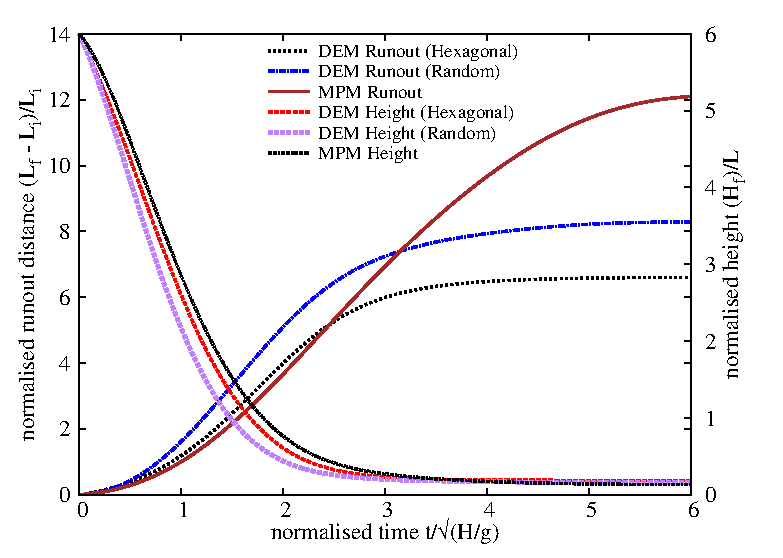
\includegraphics[width=\textwidth]{flowa6}
\caption{Flow evolution of a column with $`a'=6$}
\label{fig:flowa6}
\end{subfigure}
\caption{Flow evolution of granular column collapse}
\label{fig:flow_column}
\end{figure}

\subsection{Energy dissipation mechanism}
\label{sec:energy}
The time evolution of the flow exhibited three distinct stages during the 
collapse of a granular column. Studying the energy dissipation mechanism 
provides useful insight into the flow dynamics. %TODO: Add figure label
shows 
the time evolution of potential energy $(E_{p})$ and kinetic energy $(E_{k})$ 
normalized by the initial potential energy $E_{o}$.
\begin{align}
& 
\textit{E}_{\textit{p}}=\sum\limits_{\textit{p}=1}^{\textit{N}_{p}}{\textit{m}_{p}\textit{g}\textit{h}_{p}}
 \\
& 
\textit{E}_{\textit{ki}}=\frac{1}{2}\sum\limits_{\textit{p}=1}^{\textit{N}_{p}}{\textit{m}_{p}\textit{v}_{\textit{p}}^{2}}
\end{align}
where $\textit{N}_{p}$ is the total number of particles, $\textit{m}_{p}$ is 
the mass of a particle `\textit{p}', $\textit{h}_{p}$ is the height and 
$\textit{v}_{p}$ is the velocity of the particle `\textit{p}'. It can be 
observed from the figure that the initial potential energy stored in the 
particle is converted to kinetic energy which is dissipated as the granular 
material flows down. Three successive stages can be identified in the granular 
column collapse. In the initial acceleration stage $(\textit{t}<0.8\tau_{c})$, 
the initial potential energy stored in the grains is converted into vertical 
motion. In the second stage, the grains undergo collisions with the bottom 
plane and/or with neighbouring grains, and the stored potential energy is 
converted into horizontal motion. In the third stage, the grains eventually 
leave the base area of the column and flow sideways. As the process involves 
collective dynamics of all the particles, it is difficult to predict the exact 
trajectory of a grain, however, the overall dynamics can be explained. To 
explain the dissipation of energy during the collapse,~\citet{Staron2005} 
assumed that the total initial potential energy stored in the system is 
completely dissipated through friction over the entire run-out distance as:
\begin{align}
\mu \textit{m}_{o}g \times (L_{f}-L_{i}) = \textit{m}_{o}g \textit{H}_{o}
\end{align}
where $\mu$ is the friction coefficient. The model predicts well the flow 
dynamics for columns with larger aspect ratios, as most of the initial 
potential energy is dissipated during the collapse involving the entire column. 
However, for columns with smaller aspect ratios, only a portion of the mass 
above the failure surface is involved in the flow. Hence, the energy 
dissipation should involve only the grains lying above the failure surface. A 
mathematical model, which considers the grains lying above the failure surface, 
will be derived to predict the flow dynamics of the granular column collapse 
for different aspect ratios. 

\begin{figure}[tbhp]
\centering
\begin{subfigure}[b]{0.975\textwidth}
\includegraphics[width=\textwidth]{a04_energy}
\caption{Energy evolution of a column with $`a'=0.4$}
\label{fig:a04_energy}
\end{subfigure}
\\
\begin{subfigure}[b]{0.975\textwidth}
\centering
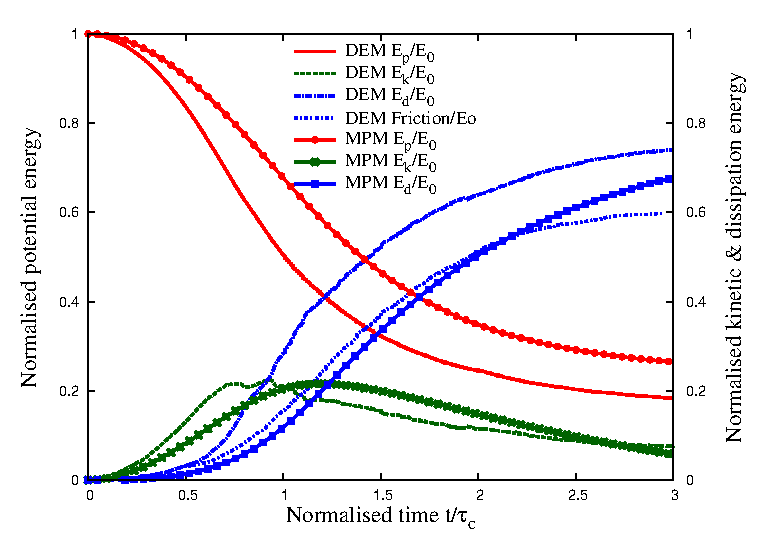
\includegraphics[width=\textwidth]{a6_energy}
\caption{Energy evolution of a column with $`a'=6$}
\label{fig:a6_energy}
\end{subfigure}
\caption{Energy evolution of granular column collapse}
\label{fig:column_energy}
\end{figure}

DEM simulations provide an insight in to the flow dynamics and energy 
dissipation. For larger aspect ratios, the flow is still initiated by a well 
defined failure surface. However, the centre of gravity of the granular column 
is much higher than the top of the failure surface, which results in free fall 
of grains under gravity consuming the column along their way. When they reach 
the vicinity of the failure surface, the grains undergo collisions with the 
bottom plane and the neighbouring grains, thus causing the flow to deviate 
along the horizontal direction releasing a large amount of kinetic energy 
gained during the free fall (see Figure~\ref{fig:a6f}). The grains then 
eventually leave the base area of the column and flow sideways undergoing 
frictional dissipation. The process involves collective dynamics of all the 
particles, and DEM simulations model both collisional and frictional 
dissipation process. However, MPM simulations assume that the total initial 
potential energy stored in the system is completely dissipated through friction 
over the entire run-out distance, resulting in larger run-out distance.

\begin{figure}[tbhp]
\centering
\begin{subfigure}[b]{0.975\textwidth}
\includegraphics[width=\textwidth]{flowa04muI}
\caption{Flow evolution of a column with $`a'=0.4$ using $\mu(I)$ rheology}
\label{fig:flowa04muI}
\end{subfigure}
\\
\begin{subfigure}[b]{0.975\textwidth}
\centering
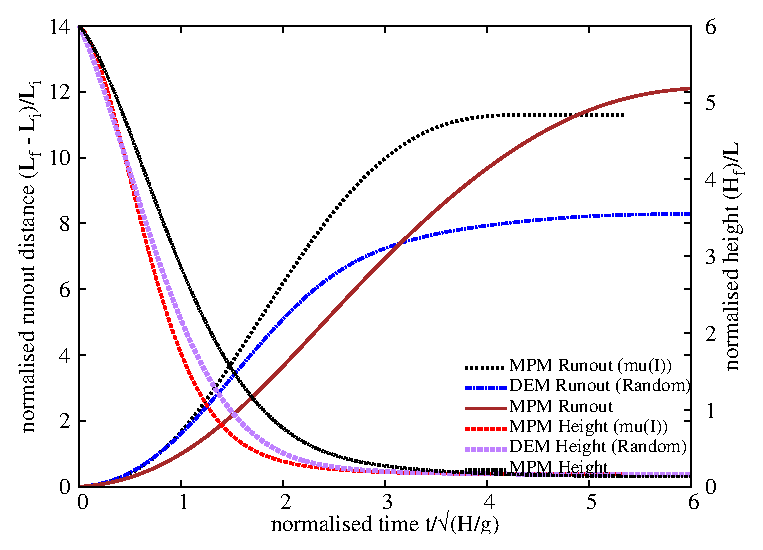
\includegraphics[width=\textwidth]{flowa6muI}
\caption{Flow evolution of a column with $`a'=6$ using $\mu(I)$ rheology}
\label{fig:flowa6muI}
\end{subfigure}
\caption{Flow evolution of granular column collapse using $\mu(I)$ rheology}
\label{fig:flow_muI}
\end{figure}

\begin{figure}[tbhp]
\centering
\includegraphics[width=\textwidth]{muI}
\caption{Evolution of inertial number with time for columns with $`a'=0.4$ and 
$`a'=6$}
\label{fig:muI}
\end{figure}

\subsection{Role of initial grain properties}

\citet{Lube2005} observed that the run-out distance scales with the initial 
aspect ratio of the column, independent of the material properties. The run-out 
evolution after the initial transition regime is a frictional dissipation 
process, and the lack of influence of material properties on the run-out 
behaviour is inconsistent with continuum modelling of granular flow behaviour. 
~\citet{Balmforth2005} observed that the material properties has almost no 
influence on the exponent of the normalised run-out as a function of the 
initial aspect ratio. The numerical constant of proportionality, however, 
showed clear material dependence. This corroborates the conclusions 
of~\citet{Lajeunesse2004} and softens that of~\citet{Lube2005}. 
~\citet{Daerr1999} observed 
the strong influence of initial packing density and the internal structure on 
the behaviour of granular flows. 


It should be noted that the collapse experiment is
highly transient and no clear stationary regime was ob
served. On the contrary, the acceleration and the deceleration 
phases cover 
nearly the whole duration of the
spreading. This makes the analysis of the structure of
the flow and its relation with other characteristic of the
system uneasy.
Considering this, we were able to show nevertheless
how the initial condition was dominating the behaviour
of the spreading through the mass distribution induced
in the flow. This means that the knowledge of the final
run-out is not a sufficient characterization of the deposit:
one also needs to know how mass is distributed to under-
stand the dynamics and the dissipation process. This is
expected to be true in natural contexts as well as in
experiments.
While the inter-grain friction
$\mu$
does not affect the early vertical dynamics, nor the power-law dependence,
it controls the effective frictional properties of the flow,
and its internal structure. It is interesting to note that
the details of the structure of the flow do not influence
the final run-out dependence, and thus seem to play a
marginal role in the overall behaviour of the spread-
ing. This could explain why simple shallow-water model
with basic rheology but where the free-fall dynamics was
accounted for could reproduce the run-out scalings.

At this stage, it appears that the collapse experiment
for large aspect ratios mixes two very different dynam-
ics: while the second stage consists of a ``conventional''
horizontal granular flows, the first stage implies a large
vertical acceleration. It shows how the initial condition
can influence the overall behaviour of a granular
system, and suggests that triggering mechanisms play a
crucial role in the case of natural flows. This stresses
the necessity of accounting for vertical acceleration in
continuum models in the perspective of producing realistic prediction of the 
behaviour of granular flows.

The numerical constants of proportionality, however, show clear material 
dependence. This corroborates the conclusion 
of~\citet{Lajeunesse2004,Balmforth2005} and 
softens that of~\citet{Lube2005}.

\begin{figure}[tbhp]
\centering
\includegraphics[width=\textwidth]{runout_height_dense_r18}
\caption{Effect of density on run-out evolution $`a' = 0.8$}
\label{fig:runout_height_dense_r18}
\end{figure}

\begin{figure}[tbhp]
\centering
\begin{subfigure}[b]{0.75\textwidth}
\centering
\includegraphics[width=\textwidth]{Energy_dense_r18}
\caption{Evolution of potential and kinetic energy}
\label{fig:Energy_dense_r18}
\end{subfigure}
\\
\begin{subfigure}[b]{0.75\textwidth}
\centering
\includegraphics[width=\textwidth]{KExy_dense_r18}
\caption{Effect of kinetic energy}
\label{fig:KExy_dense_r18}
\end{subfigure}
\caption{Effect of density on energy evolution $a = 0.8$}
\label{fig:Energy_density_r18}
\end{figure}


\begin{figure}[tbhp]
\centering
\includegraphics[width=\textwidth]{voro_r18}
\caption{Evolution of local packing density $`a' = 0.8$}
\label{fig:voro_r18}
\end{figure}

\begin{figure}[tbhp]
\centering
\includegraphics[width=\textwidth]{runout_height_dense_r6}
\caption{Effect of density on run-out evolution $`a' = 0.8$ (poly-dispersity 
`r' = 6)}
\label{fig:runout_height_dense_r6}
\end{figure}


\begin{figure}[tbhp]
\centering
\begin{subfigure}[b]{\textwidth}
\centering
\includegraphics[width=\textwidth]{dense_a08_r6_final}
\caption{Dense initial packing}
\label{fig:dense_a08_r6_final}
\end{subfigure}
\\
\begin{subfigure}[b]{\textwidth}
\centering
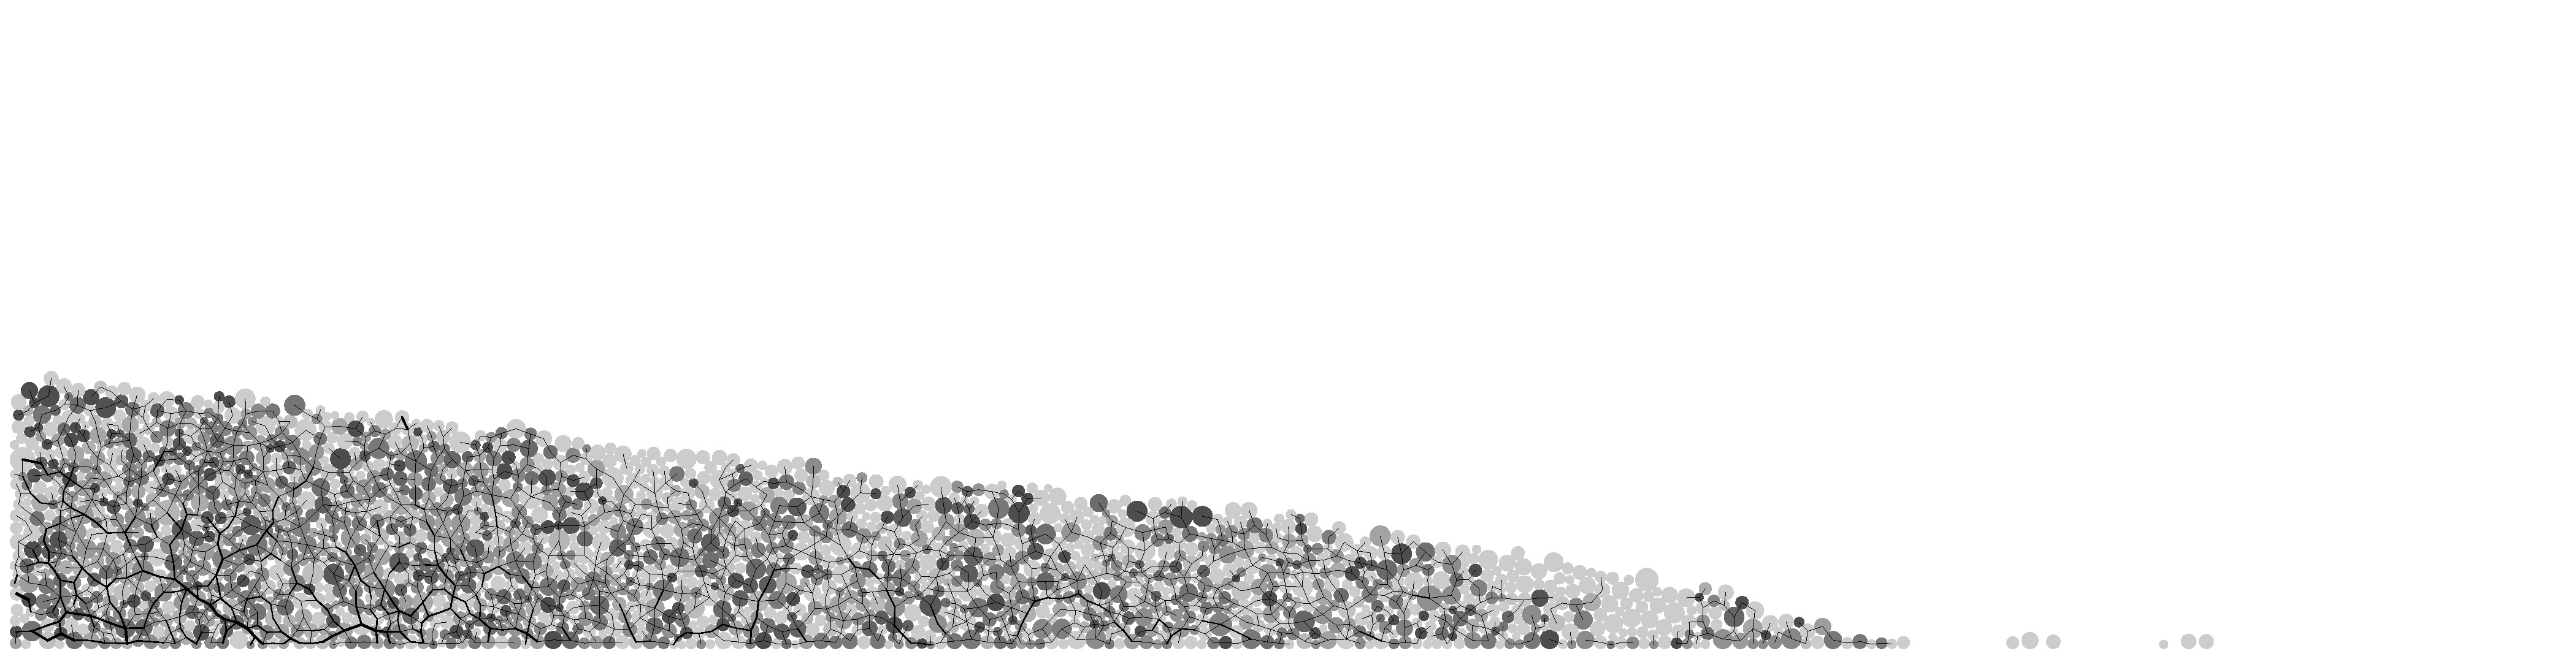
\includegraphics[width=\textwidth]{loose_a08_r6_final}
\caption{Loose initial packing}
\label{fig:loose_a08_r6_final}
\end{subfigure}
\caption{Snapshots of granular column collapse $t = 6 \tau_c$}
\label{fig:density_r6}
\end{figure}


\begin{figure}[tbhp]
\centering
\begin{subfigure}[b]{0.75\textwidth}
\centering
\includegraphics[width=\textwidth]{Energy_dense_r6}
\caption{Evolution of potential and kinetic energy}
\label{fig:Energy_dense_r6}
\end{subfigure}
\\
\begin{subfigure}[b]{0.75\textwidth}
\centering
\includegraphics[width=\textwidth]{voro_r6}
\caption{Evolution of packing density}
\label{fig:voro_r6}
\end{subfigure}
\caption{Effect of density on energy and packing fraction evolution $`a' = 0.8$ 
(poly-dispersity `r' = 6)}
\label{fig:Energy_voro_r6}
\end{figure}


\begin{figure}[tbhp]
\centering
\begin{subfigure}[b]{0.95\textwidth}
\includegraphics[width=\textwidth]{runout_height_dense_a6}
\caption{Effect of density on run-out evolution}
\label{fig:runout_height_dense_a6}
\end{subfigure}
\\
\begin{subfigure}[b]{0.95\textwidth}
\centering
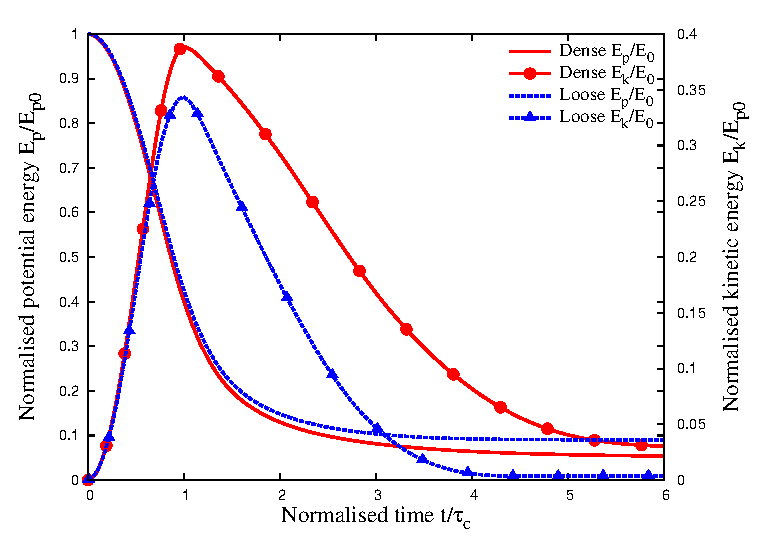
\includegraphics[width=\textwidth]{Energy_dense_a6}
\caption{Effect of density on energy evolution}
\label{fig:Energy_dense_a6}
\end{subfigure}
\caption{Effect of density on run-out behaviour and energy evolution $`a' = 
0.6$}
\label{fig:Density_a6}
\end{figure}

\section{Slopes subjected to impact loading}


Transient granular flows occur very often in nature. 
Well-known examples are rockfalls, debris flows, 
and aerial and submarine avalanches. They form a major element of 
lanscape reshape and their high destructive potential is a 
substantial factor of risk. Natural granular flows may be triggered 
as a result of different processes such as gradual degradation,   
induced by weathering or chemical reactions, liquefaction    
and external forces such as earthquakes.          

Granular flows have been studied in laboratory experiments in different 
geometries such as tilted piles leading to slope failure and surface avalanches 
\citep{Legros2002, Iverson1997} or by considering vertical columns 
of grains collapsing and spreading under their own weight 
\citep{Lajeunesse2004, 
Lajeunesse2005}. The dynamics observed in the experiments is often nontrivial 
in the sense that the final configurations after the dissipation of the whole 
kinetic energy  
can not be readily predicted by means of simple laws based on the Mohr-Coulomb 
nature 
of the material. For example, in collapsing columns, the run-out distance 
is found to obey a power-law dependence upon the initial aspect ratio of the 
column. 

The observed nontrivial transient dynamics is often correctly 
reproduced by the DEM, which provides 
a powerful tool for the grain-scale analysis of the 
trigger and its subsequent dynamics \citep{Staron2005, Staron2009}. 
However, even in simplified geometries such as those 
investigated in the experiments, the DEM suffers from a serious 
short-coming in the number of particles that can be simulated in 
a reasonnable time. This is a critical issue when more complex geometries or 
long-time granular processes are considered, or when particle size 
distributions are broad. For this reason, most numerical studies 
are performed in 2D or simple particles shapes and size distributions 
are considered. 

It is also obvious that classical modelling strategies based on 
the finite element method (FEM) cannot be used for the 
simulation of very large deformations. In various application of FEM, 
this problem is treated by means of technical tools such 
as re-meshing. Such mthods are, however, not robust and lead 
to round-off errors and mesh-senstitivity. In contrast, the so-called 
Material Point Method (MPM) is an alternative approach for 
continuum problems that allows for indefinitely large deformations 
without re-meshing \cite{Sulski??}. In this method, the material points carry 
the information 
on state variables and a background fixe grid is used to solve the governing 
equations. 
The information between the material points and the grid is exchanged via 
suitable shape functions. The MPM has been applied with success to 
a number of solid mechanics problems and its theoretical foundations 
have recently been investigated by several authors. 

In this paper, we are concerned with the ability of the MPM, as a continuum 
approach, to reproduce the evolution of a granular pile 
under its own weight or when destabilized by energy input. In particular, 
a central issue is whether power-law dependence of the run-out distance 
and timew ith respect to the initial geometry or energy can be reproduced 
by a simple prescription of the Mohr-Coulomb plastic behaviour within a  
MPM code. We therefore perform extensive simulations by varying continuously 
different input parameters and compare the data with those obtained from 
DEM simulations of the same system. We compare in detail the evolution of 
the profile of the pile and its total kinetic energy between the two methods 
and for different initial states. As we shall see, the MPM can successfully 
simulate the transient evolution with a single input parameter, namely the 
internal angle of friction. This opens the way to the simulation of 
geological-scale flows on complex topographies.  
  

\subsection{Numerical procedures}
\label{sec:num}

The numerical samples are composed of $\sim13000$ disks with a uniform 
%plus de simulation pour faire une moyenne ($\sim 6$)
distribution of diameters by volume fractions in the range $[d_{min}, 
d_{max}]$ with $d_{max} = 1.5 d_{min}$. The mean particle diameter and 
mass are $d\simeq 0.0025 $ m and $m\simeq 0.0123$ kg, respectively. 
The particles are first poured uniformly into a rectangular box of given width 
and then the right-hand side wall is shifted further to the right to allow the 
particles to spread. A half-pile is obtained when all particles come to 
rest; see ~\cref{fig:Initial_final_configuration}. This procedure leads to 
a 
mean packing fraction $\simeq 0.83$.

%\begin{figure}
%\centerline{
%\resizebox{0.5\textwidth}{!}{%
% 	 \includegraphics{Figures/Initial_final_configuration}
%}}
%\caption{Initial geometry and dimensions of the pile}
%\label{fig:Initial_final_configuration}
%\end{figure}


\begin{table}[tbhp]
\caption{DEM simulation of simple shear test~\citep{Mutabaruka2013}}
\label{table:CD_Shear}
\centering
\begin{tabular}{ll}
\toprule
\textbf{Parameter} & \textbf{Value} \\ \midrule
Mean grain diameter & $\approx 2.455$~\si{\mm} \\
Grain diameter $[d_{min}:d_{max}]$ & [2.0, 3.0]~\si{\mm} \\
Friction coefficient & 0.4\\
Grain density & 2600\si{\kg\per\meter\cubed} \\
Restitution coefficient  & $0$\\
Number of grains & 1174 \\
\bottomrule
\end{tabular}
\end{table}


The initial static pile is set into motion by applying a constant horizontal
gradient  $v_{0x}(y) = k (y_{max} - y)$ with $k>0$. Such a configuration 
mimics the energy transfer mechanism of a horizontal quake along the bottom of 
the pile. We are interested in the evolution of the geometry of the pile 
and its total kinetic energy as a function of the initial input energy $E_0$. 
The run-out distance $R_f$ is the distance of the rightmost particles 
from the left wall when the pile comes to rest.  It will be normalized by the 
initial extension $R_0$ of the pile, as in the experiments of collapsing 
columns. The total run-out duration $t_f$ is the time that the pile takes to 
reach its final run-out distance $R_f$.

The initial static pile is set into motion by applying a horizontal velocity 
$v_{0x}(y)$ to all particles during a short interval of time. Different 
velocity fields were tested: 1) The same velocity $v_{0x}(y) = v_0$ applied to 
all particles, 2) The same velocity $v_{0x}(y) = v_0$ applied to a column of 
particles next to the left wall, 3) a constant velocity gradient  $v_{0x}(y) = 
k (y_{max} - y)$ with $k>0$. The first two pushing modes mimic the case of a 
pile impacted from the left by a moving mass (tsunami, debris\dots) whereas the 
last mode represents energy transfer by horizontal quake of the bottom line. We 
will compare briefly below the effect of different pushing modes, but later we 
will mainly explore the third mode. We are interested in the evolution of the 
geometry of the pile and its total kinetic energy as a function of the initial 
energy input $E_0$. The run-out distance $R_f$ is the distance of the rightmost 
particles from the left wall when the pile comes to rest.  
It will be normalized by the initial extension $R_0$ of the pile, as in 
the experiments of collapsing columns. The total run-out duration $t_f$ is the 
time that the pile takes to reach its final run-out distance $R_f$.       

For grain scale simulations, classical DEM and Contact 
Dynamics approach is used. 
A detailed description of the Contact Dynamics 
method can be found in \cite{Moreau1993,Jean1999,Radjai2009,Radjai2011}. 
This method is based on implicit time integration of the equations of motion 
and a nonsmooth formulation of mutual exclusion and dry friction between 
particles. The CD method requires no elastic repulsive potential and no 
smoothing of the Coulomb friction law for the determination of forces. 
For this reason, the simulations can be performed with large time steps 
compared to discrete element simulations. The unknown variables are particle 
velocities and contact forces, which are calculated at each time step by taking 
into account the conservation of momenta and the constraints due to mutual 
exclusion between particles and the Coulomb friction. We use an iterative 
research algorithm based on a nonlinear Gauss-Seidel scheme. The only contact 
parameters within the CD method are the friction coefficient $\mu_s$, the 
normal restitution coefficient $e_n$ and the tangential restitution coefficient 
$e_t$ between particles. We will investigate the effect of these parameters on 
the evolution of kinetic energy and the profile of the pile.     
  
The natural units of our system are the mean particle diameter $d$, 
mean particle mass $m$ and gravity $g$. For this reason, 
in the following we normalize the lengths by $d$, the times by $(d/g)^{1/2}$, 
the velocities by $(gd)^{1/2}$ and the energies by $mgd$.

\begin{figure}[tbph]
\centering
\begin{subfigure}[t]{0.475\textwidth}
\includegraphics[width=0.95\textwidth]{Sxy_vs_Syy_Slope}
\caption{Evaluating the critical state friction angle from periodic shear 
test.}
\label{fig:Sxy_vs_Syy_Slope}
\end{subfigure}
%
\begin{subfigure}[t]{0.475\textwidth}
\includegraphics[width=0.95\textwidth]{mu_vs_I}
\caption{Evolution of Inertial number with friction $\mu$}
\label{fig:mu_vs_I}
\end{subfigure}
\caption{Periodic shear test using CD~\citep{Mutabaruka2013}.}
\label{fig:Shear_Test_Slope}
\end{figure}

%-------------------------------------------------------------------------------
\subsection{Evolution of pile geometry and run-out}
\label{sec:evolution}

In this section, we consider the spreading process following the initial energy 
input into the pile. Fig. \ref{fig:quake_mod} shows several snapshots of the 
pile for an initial input energy $E_0 = 61$ (in dimensionless units).
The pile is sheared from the bottom to the top, thus leaving a cavity in the 
vicinity of the left wall. The cavity is partially filled while the pile 
continues to spread to the right. 


In this section, we consider the spreading process 
following the initial energy input into the pile. 
Fig. \ref{fig:quake_mod} shows several snapshots of the pile 
for each pushing mode and for the same initial 
energy $E_0 = 61$ (in dimensionless units). 
In mode 1, where the same velocity is imparted to 
all particles, the whole pile moves away  from 
the left wall over a short distance and then it 
spreads out and declines in slope. 
 The spreading continues farther until the slope nearly 
declines to zero. In mode 2, where the velocity is applied to 
a  column of particles next to the left wall, the particles belonging to 
the column are literally expelled from the pile. They fall back farther way on 
the pile after 
a ballistic travel above the pile. At the same time, the right side of the 
pile slightly spreads away  
while the left side is filled by the particles rolling down into the gap 
left by the column. In mode 3, the pile is  
sheared from the bottom to the top, leaving thus a cavity in the 
vicinity of the left wall. The cavity is partially filled while the pile 
continues to spread. 

All pushing modes involve a transient with a sharp change 
of the geometry of the pile followed by continuous spreading to the right. 
In mode 2, most of the energy is carried away by the ejected particles. 
In mode 1, the pile has a rigid-body velocity component and moves 
away from the left wall, but shows an efficient energy transfer leading to a 
long run-out distance.      
The transient is more energy consuming in  mode 3  compared to 
mode 1. For this reason, the run-out distance in mode 3 is long but shorter 
than in mode 1. In the following, we analyze in more detail 
the evolution of the pile in mode 3, which mimics a  
horizontal quake from the bottom and, despite the creation of a cavity, 
remains always in contact with the left wall irrespective of the input 
energy.   


Figure \ref{fig:run-out} shows the normalized run-out distance $(R_f - R_0)/R_0$ 
and total run-out time $t_f$ as a function of the input energy $E_0$. We observe 
two regimes both characterized by a power-law run-out distance and time as a 
function of $E_0$. In the first regime, corresponding to the range of low input 
energies $E_0 < 40 \ mgd$, the run-out distance varies as $R_f \propto 
(E_0)^\alpha$ with $\alpha \simeq 0.61 \pm 0.04$ over nearly one decade while 
the duration keeps a constant value  $t_f \simeq 60 \  (d/g)^{0.5}$ 
irrespective of the value of $E_0$! The error  on the value of the exponent 
represents the confidence interval of linear fits on the logarithmic scale.  
%lancer plus de simulation pour une  moyenne 
An average run-out speed can be defined from the ratio $v_s = (R_f - R_0) / 
t_f$. According to the data, we have $v_s \propto (E_0)^{0.61\pm 0.04}$. Since 
the initial average velocity varies as $v_0 \propto (E_0)^{0.5}$, this 
difference between the values of the exponents suggests that the mobilized mass 
during run-out declines when the input energy is increased. As we shall see 
below, the constant run-out time reflects also the collapse of the particles 
into the cavity left behind the pile. 

In the second regime, corresponding to the range of high input energies  $E_0 > 
40 \ mgd$, the run-out distance varies as $R_f \propto (E_0)^{\alpha'}$ over one 
decade with $\alpha' \simeq 0.77\pm 0.03$ while the duration increases as $t_f 
\propto (E_0)^{\beta'}$ with $\beta' \simeq 0.21 \pm 0.04$. Hence, in this 
regime the average run-out speed varies as $v_s \propto (E_0)^{0.56 \pm 0.07}$. 
This exponent is close to the value $0.5$ in $v_0 \propto (E_0)^{0.5}$, and 
hence, within the confidence interval of the exponents, in the second regime we 
may assume $\beta' \simeq \alpha' - 0.5$ and $v_s \propto v_0$. 

It is worth noting that a similar power-law dependence of the 
run-out distance and time were found in the case of 
collapsing columns of grains with respect to the initial aspect ratio 
\cite{Topin2012}.  
In the column geometry, the particles spread away owing to the 
kinetic energy acquired during gravitational collapse of the column. 
Topin et al. found that the run-out distance varies as a power law 
of the available peak kinetic energy at the end of the free-fall stage with an 
exponent $\simeq 0.5$. This value is below those obtained here 
for both regimes. This is, however, physically plausible since the   
distribution of particle kinetic energies at the end of the collapse 
is more chaotic than in our simulations where the energy is supplied 
from the very beginning in a well-defined shear mode. As pointed out 
by \cite{Staron2005}, the distribution of kinetic energies is an essential 
factor for the run-out distance.

\begin{figure}[tbph]
\centering
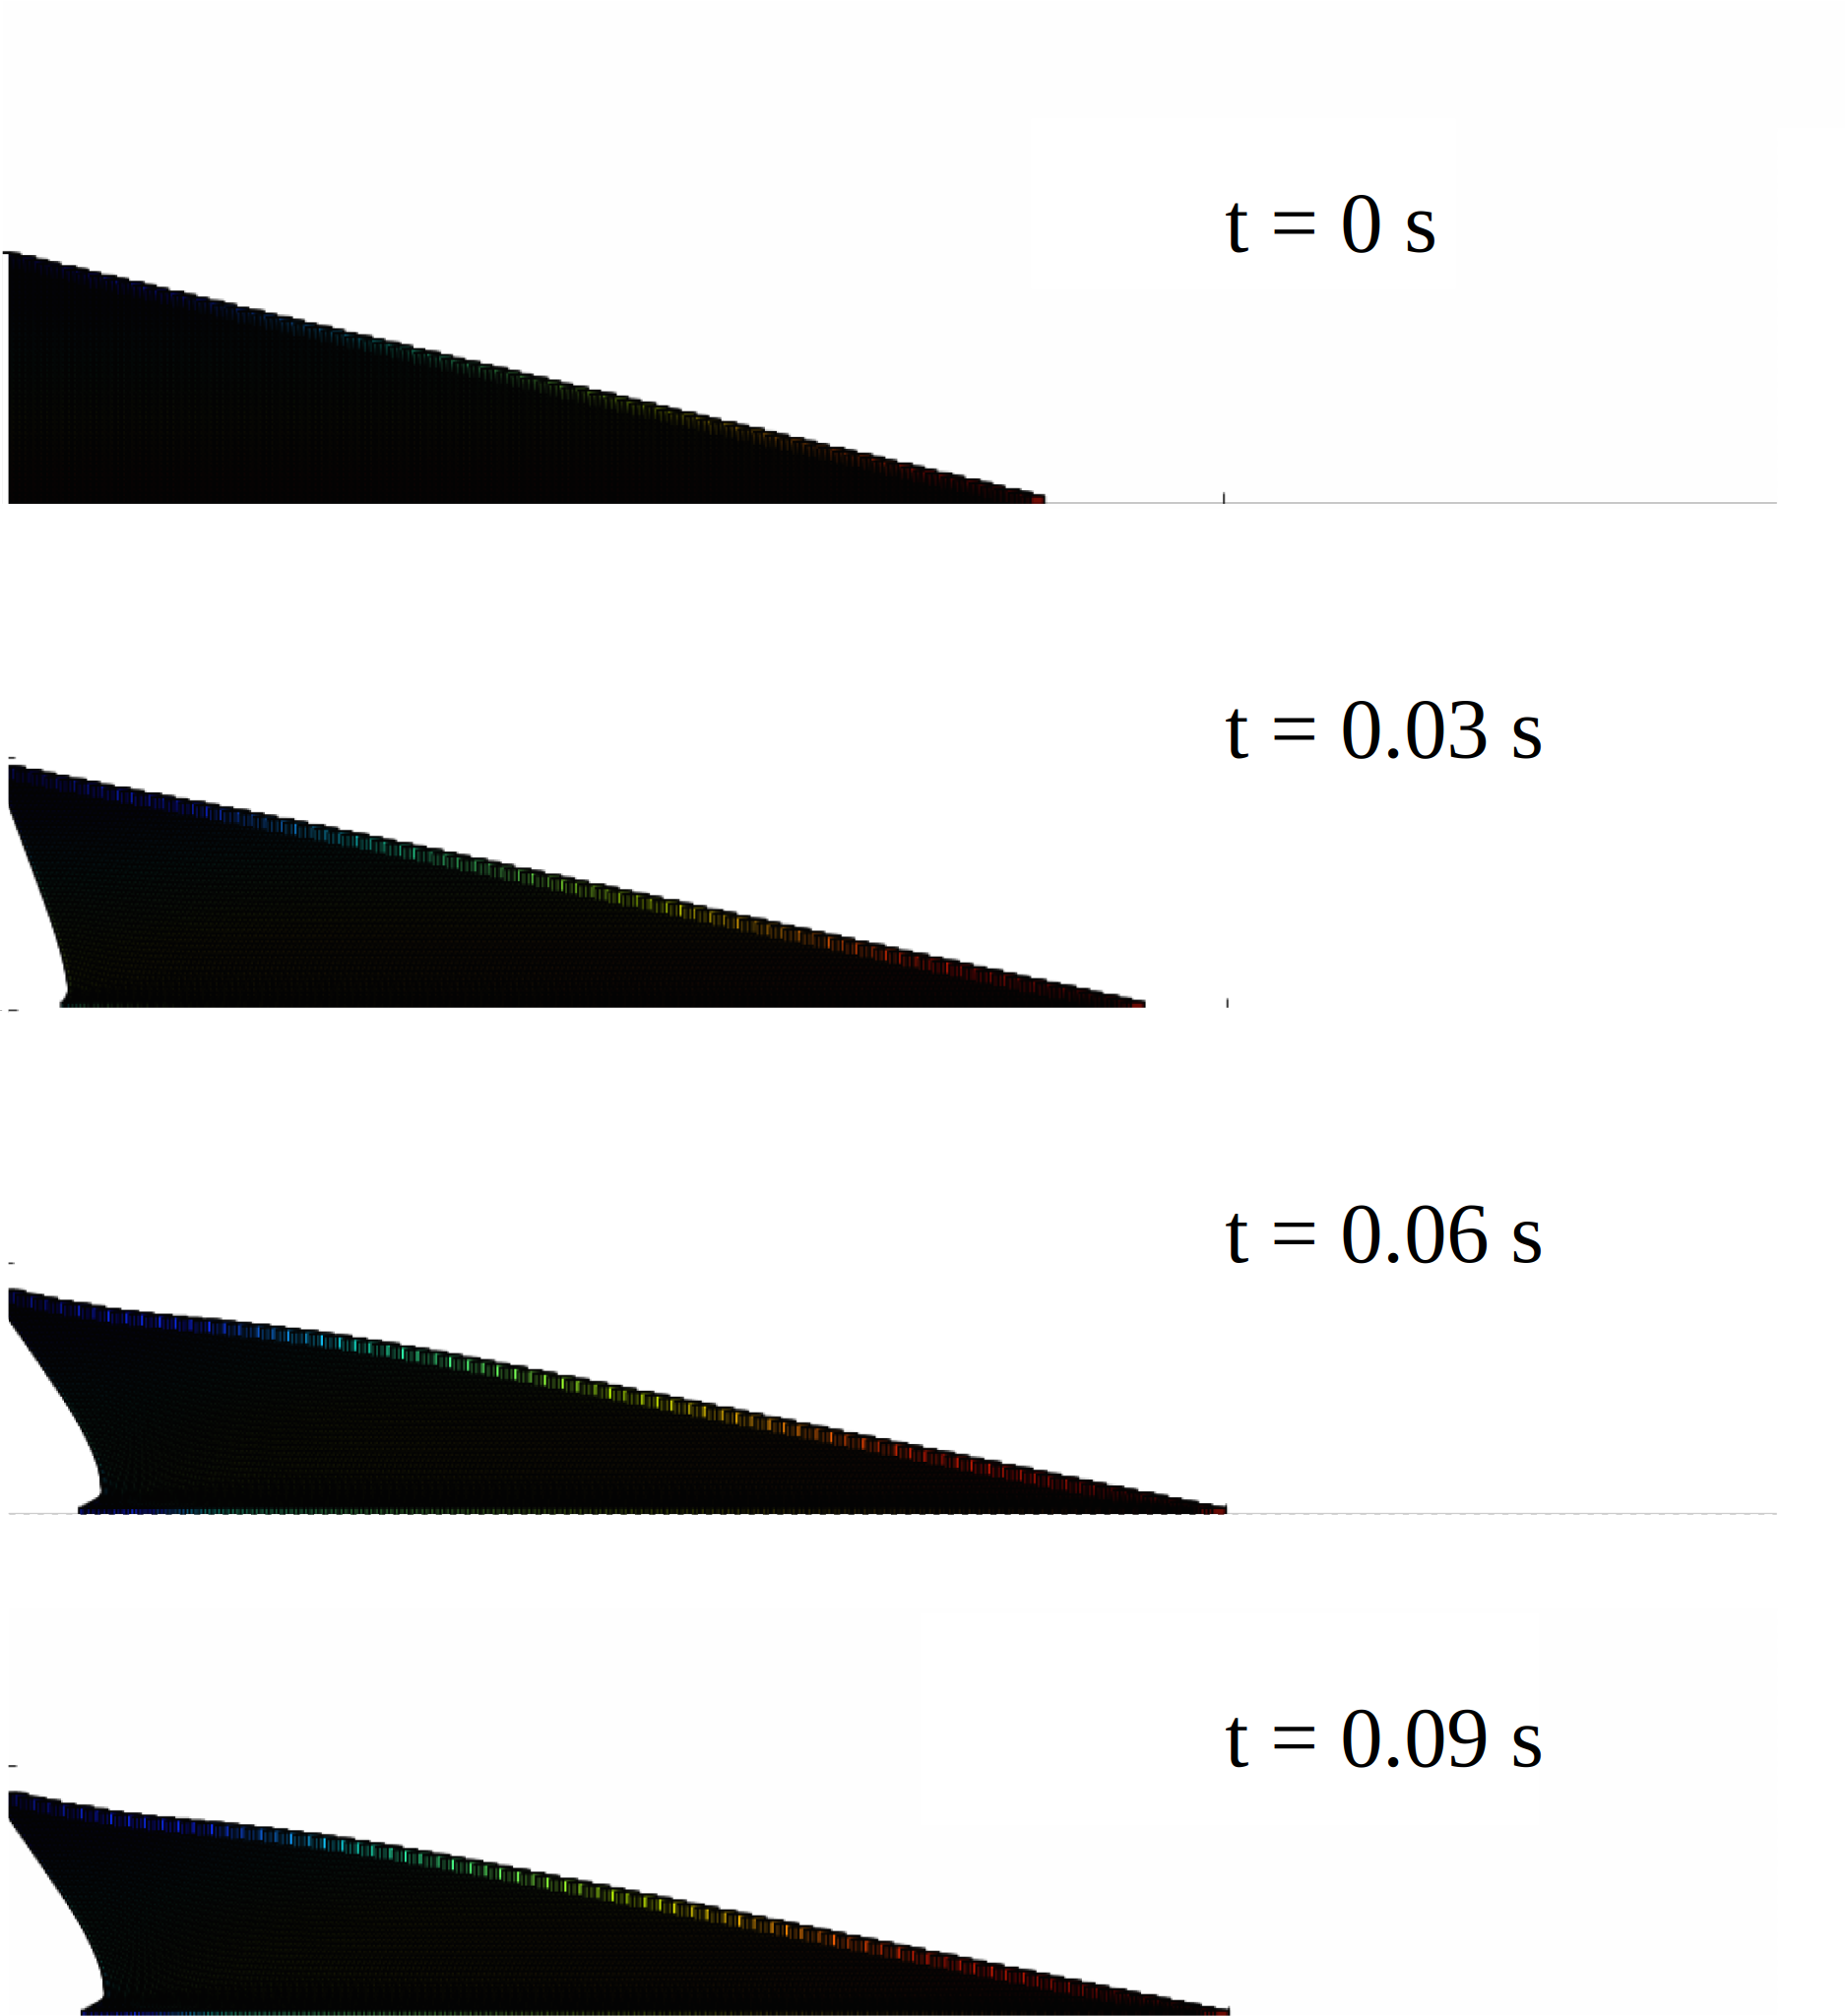
\includegraphics[width=\textwidth]{Gradient_Slope_Profile_200J}
\caption{Snapshots of MPM simulations of the evolution of granular pile 
subjected to a gradient impact energy.}
\label{fig:Gradient_Slope_Profile_200J}
\end{figure}

\begin{figure}[tbph]
\centering
\includegraphics[width=\textwidth]{Gradient_Slope_CD_200J}
\caption{Snapshots of CD simulations of the evolution of granular pile 
subjected to a gradient impact energy~\citep{Mutabaruka2013}.}
\label{fig:Gradient_Slope_CD_200J}
\end{figure}

\begin{figure}[tbph]
\centering
\begin{subfigure}[b]{0.975\textwidth}
\centering
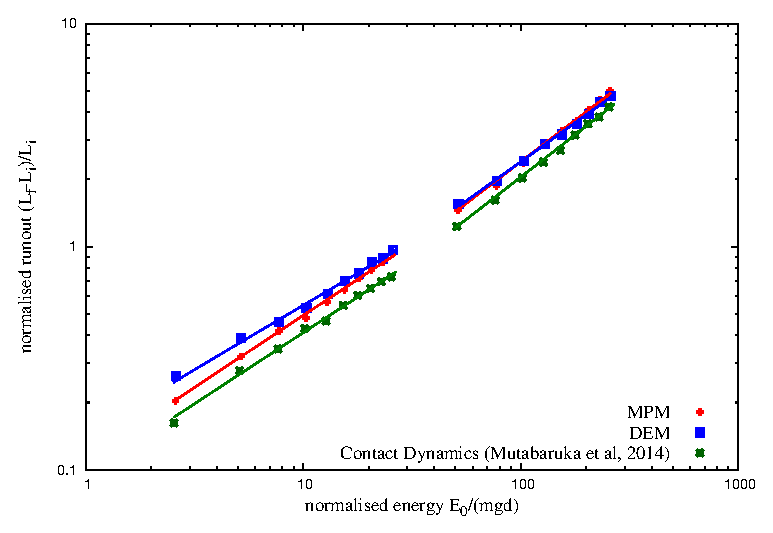
\includegraphics[width=\textwidth]{Runout_Eo_MPM_CD_DEM}
\caption{Run-out distance with normalised input kinetic energy}
\label{fig:Runout_Eo_MPM_CD_DEM}
\end{subfigure}
\\
\begin{subfigure}[b]{0.975\textwidth}
\centering
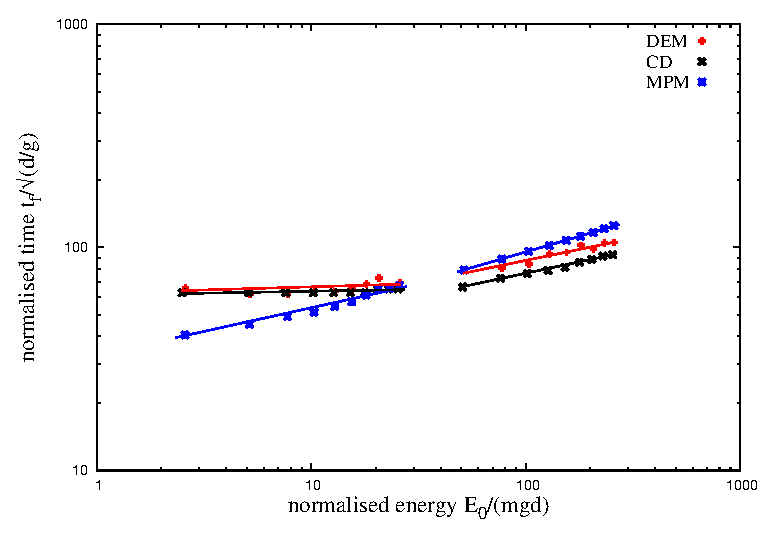
\includegraphics[width=\textwidth]{Tf_vs_Eo_Slope}
\caption{Duration of run-out with normalised input kinetic energy}
\label{fig:Tf_vs_Eo_Slope}
\end{subfigure}
\caption{Run-out behaviour of a pile subjected a gradient impact energy}
\label{fig:Slope}
\end{figure}

%-------------------------------------------------------------------------------------------
\subsection{Decay of kinetic energy}
\label{sec:decay}

The non-trivial evolution of the pile geometry  in two regimes suggests that 
the energy supplied to the pile is not simply dissipated by shear and friction 
with the bottom plane. We also need to split the kinetic energy into its 
different components ($x$, $y$ and rotation) of the velocity field. The input 
energy is in the $x$ component, but due to both the creation of a cavity next 
to the left wall and the rolling of the particles down the free surface of the 
pile and between particles, a fraction of the energy is first transferred to 
the $y$ component of the velocity field and dissipated  during the transient. 
In this section, we analyse these features  in order to arrive in a picture 
consistent with the evolution of the pile shape.  

The decay of the total kinetic energy $E$ is displayed in 
~\cref{fig:E_vs}(a) for values of the input energy $E_0$. We observe an 
initial fast drop of $E$ followed by a regular fall-off until the end of the 
run-out. This regular fall-off occurs clearly with two different functional 
forms, thus revealing two stages in the evolution of the pile. 
~\cref{fig:E_vs}(b) shows the same plots normalized by $E_0$. We see that 
all plots corresponding to the first regime (low energies) collapse nearly on 
to a single time evolution. 
%to the first regime (low energies) collapse nearly all along time evolution. 
This is consistent with the fact that, as previously shown, in this 
regime the run-out time $t_f$ is independent of the input energy. In contrast, 
the plots corresponding to the second regime (high energies) collapse only at 
the beginning of run-out, i.e. for $t < t_1 \simeq 7.5 \ (d/g)^{0.5}$.   

\begin{figure}[tbhp]
\centering
\begin{subfigure}[b]{0.975\textwidth}
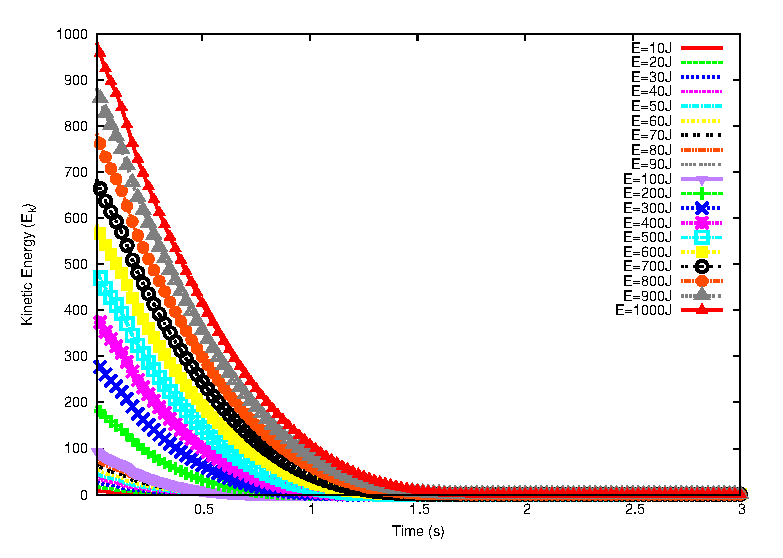
\includegraphics[width=\textwidth]{Energy_Slope}
\caption{Evolution of total kinetic energy with time}
\label{fig:energy_slope}
\end{subfigure}
\\
\begin{subfigure}[b]{0.975\textwidth}
\centering
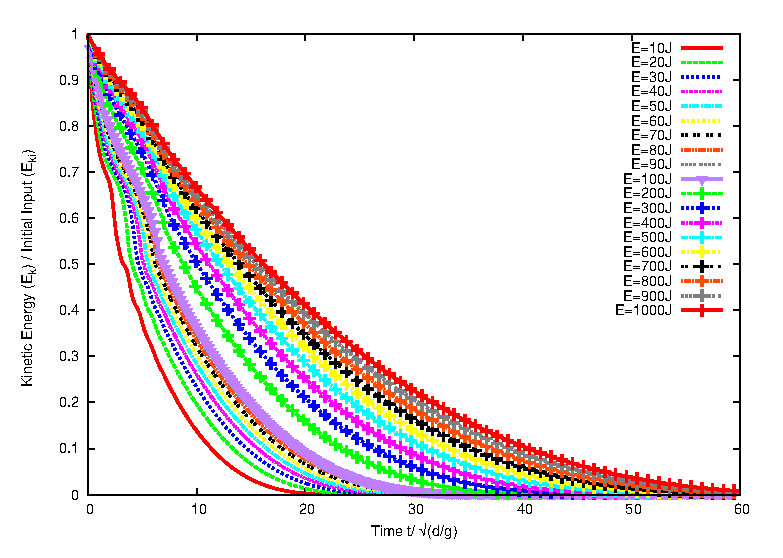
\includegraphics[width=\textwidth]{Normalised_Energy_Time_Slope}
\caption{Evolution of normalised kinetic energy with normalised time}
\label{fig:Normalised_Energy_Time_Slope}
\end{subfigure}
\caption{Evolution of kinetic energy with time}
\label{fig:Energy_Time_Slope}
\end{figure}

~\Cref{fig:E_xyt_vs_t} displays the evolution of kinetic energy 
in the translational ($E_x$ and $E_y$) and rotational ($E_\theta$) 
degrees of freedom of the particles. $E_x$ decays as the total 
energy, but $E_y$ and $E_\theta$ increase and pass through a peak before 
decaying rapidly to a negligibly small level. The transient is best observed 
for $E_y$, which has significant values only for $t< t_1$. This energy 
represents the proportion of kinetic energy transferred to the $y$ component of 
the velocity field  due to the destabilization of the pile and collapse of 
particles in the cavity behind the pile. We note that the lower $E_0$, the 
higher the peak value of $E_y/E_0$. 
%mettre une flèche sur les courbes pour montrer la décroissance de E_0
This means that, at low values of the input energy a larger fraction 
of input energy $E_0$ is consumed in the destabilization process whereas 
at a high level of input energy, most of it is dissipated in the spreading 
phase. For this reason, the total duration $t_1$ of this destabilization 
transient is nearly the same in both regimes and its value is controlled by the 
gravity rather than the input energy. The height of the pile being of the order 
of $80 \ d$, the total free-fall time for a particle located at this height is 
$\simeq 12 \ (d/g)^{0.5}$, which is of the same order as $t_1$. As to the 
rotational energy, its contribution both to the transient stage and spreading 
appears to be negligible. 

\begin{figure}[tbhp]
\centering
\begin{subfigure}[b]{0.975\textwidth}
\includegraphics[width=\textwidth]{Normalised_KEx_Slope}
\caption{Evolution of normalised horizontal kinetic energy with time}
\label{fig:Normalised_KEx_Slope}
\end{subfigure}
\\
\begin{subfigure}[b]{0.975\textwidth}
\centering
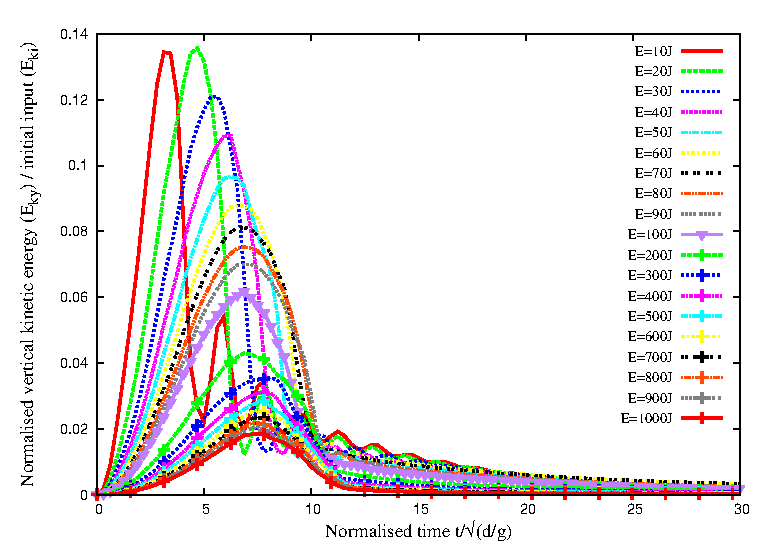
\includegraphics[width=\textwidth]{Normalised_KEy_Slope}
\caption{Evolution of normalised vertical kinetic energy with time}
\label{fig:Normalised_KEy_Slope}
\end{subfigure}
\caption{Evolution of vertical and horizontal kinetic energy with time}
\label{fig:Normalised_KEx_KEy_Slope}
\end{figure}

To analyze the second phase in the second regime, we now consider only the 
kinetic energy $E'_{x0}$ available at the end of the transient. This energy 
is responsible for most of the run-out and hence it is expected to control the 
run-out distance and time. Fig. \ref{fig:ExoEx0_vs_t_totau}(a) shows the 
evolution of $E_x$ normalized by $E'_{x0}$ as a function of time. The plots 
have seemingly the same aspect but they show different decay times. A decay 
time $\tau$ can be defined as the time required for $E_x$ to decline by a 
factor $1/2$. Fig. \ref{fig:ExoEx0_vs_t_totau}(b) shows the same data in which 
the time $t'$ elapsed since $t_1$ is normalized by $\tau$. Interestingly, now 
all the data nicely collapse on the same curve. We checked that this curve can 
not be fitted by simple functional forms such as variants of exponential decay. 
This means that the spreading of the pile is not a self-similar process in 
agreement with the fact that the energy fades away in a finite time $t'_f$. 


\begin{figure}[tbhp]
\centering
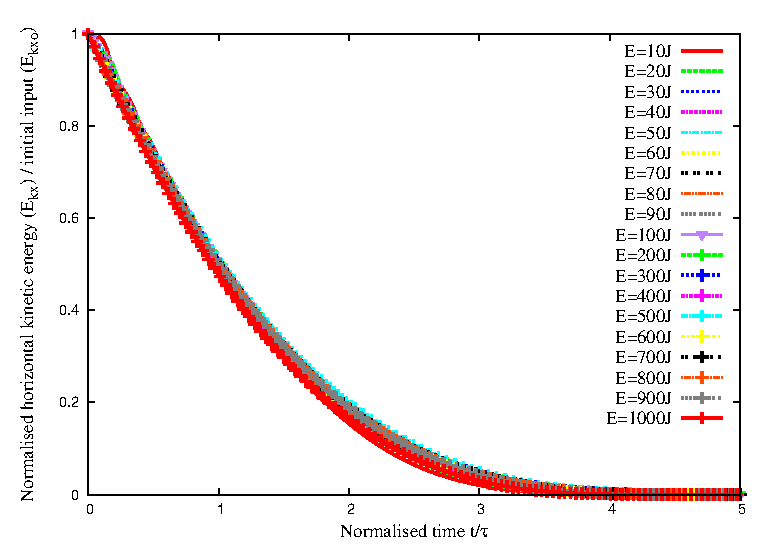
\includegraphics[width=\textwidth]{EkxKoTTau_Slope}
\caption{Evolution of kinetic energy in the $x$ component of 
the velocity field  normalized by the available kinetic energy at the end of 
the transient as a function of normalized time.}
\label{fig:ExEx0_vs_ttau}
\end{figure}


The scaling of the data with the decay time $\tau$ suggests also that the 
run-out time $t'_f$ since the beginning of the second phase might be a simple 
function of $\tau$.~\Cref{fig:ExEx0_vs_ttau} shows both $t'_f$ and $\tau$ as 
a function of $E'_{x0}$, where we observe a power law for both times over 
nearly one decade. The run-out time $t'_f \propto (E'_{x0})^{\beta'}$ has the 
same exponent $\beta' \simeq 0.21 \pm 0.03$ as $t_f$ as a function of $E_0$ 
(see Fig. \ref{fig:run-out}). For the decay time we have 
$\tau \propto (E'_{x0})^{\beta''}$ with $\beta'' \simeq 0.28 \pm 0.03$. The 
relation between the two times can thus be expressed as 
\begin{equation}
t'_f = k  \ \tau \, (E'_{x0})^{\beta'' - \beta'}, 
\label{eqn:t'f}
\end{equation}
where $k \simeq 5 \pm 0.4$ and $\beta'' - \beta' \simeq -0.05 \pm 0.06$. This 
value is small enough to be neglected within the confidence interval of our 
data. It is therefore plausible to assume that  the run-out time is a multiple 
of the decay time and the spreading process is controlled by a single time. We 
however note that a weak dependence on the energy $E'_{x0}$  is consistent with 
the fact that the whole available energy at the beginning of the second phase 
is not dissipated in the spreading process (calculated from the position of the 
tip of the pile) since  the pile keeps deforming by the movements of the 
particles at the free surface even when the tip comes to rest. 
This can explain the small difference between the two exponents as observed 
here.


\begin{figure}[tbhp]
\centering
\begin{subfigure}[b]{0.975\textwidth}
\includegraphics[width=\textwidth]{tp_tau_mgd}
\caption{Power law evolution of $t'_f$ and $\tau$ as a function of kinetic 
energy $E_{kx0}$.}
\label{fig:tp_tau_mgd}
\end{subfigure}
\\
\begin{subfigure}[b]{0.975\textwidth}
\centering
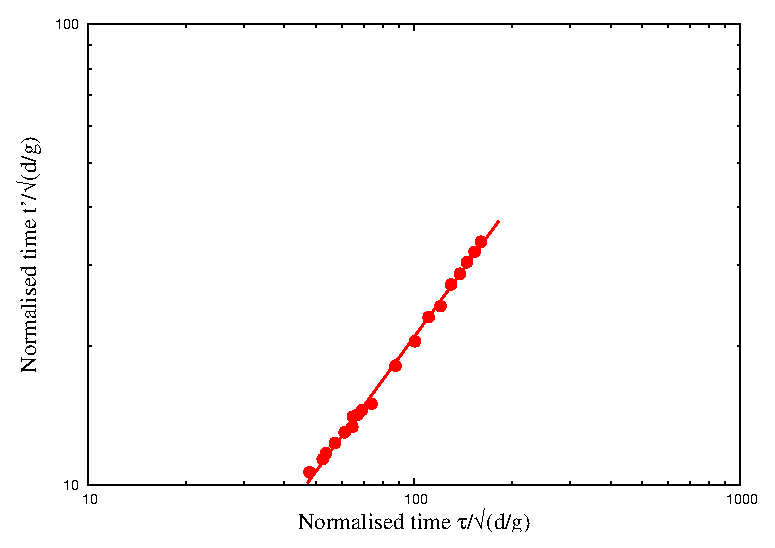
\includegraphics[width=\textwidth]{tpTau}
\caption{Linear relationship between decay time and run-out time after the 
transient as a function of the normalised kinetic energy $E_{kx0}$.}
\label{fig:tpTau}
\end{subfigure}
\caption{Decay time and run-out time as a function of the normalised kinetic 
energy $E_{kx0}$.}
\label{fig:tp_Tau}
\end{figure}


%------------------------------------------------------------------------------------
\subsection{Effect of friction}
\label{sec:parameters}

The run-out distance and time and the dissipation of kinetic energy are 
controlled by the input energy and collective dynamics of the whole pile, as it 
was analyzed in the previous sections. But they are expected to depend also on 
the friction. We performed a series of simulations with different values of 
base friction. The results are shown in Fig. \ref{fig:para} for the profiles of 
the pile and evolution of the kinetic energy in time. We see no difference in 
the results for different values of $e_n = e_t$. This is a consequence of the 
fact that,  even at large input energies, the pile remains in a dense state so 
that multiple collisions inside the pile occur at small time scales compared to 
the deformation time. When the restitution coefficients are increased, more 
collisions occur during a longer time interval but the overall energy 
dissipation rate by collisions remains the same. This effect is a seminal 
example of collective effects which erase the influence of local parameters at 
the macroscopic scale. In contrast with the restitution coefficients, however, 
the effect of the friction coefficient is quite important for the run-out, as 
observed in Fig. \ref{fig:para} for both the energy decay and geometrical 
profile of the pile. Both the run-out distance and decay time decrease as the 
friction coefficient is increased. This effect is much more pronounced at low 
values of the friction coefficient. The run-out time, for example, is reduced 
by a factor 4 as $\mu_s$ is increased from 0.1 to 0.4 while the run-out times 
and profiles do not change much for $\mu_s = 0.7$. This ``saturation effect" 
was evidenced in a systematic way in simple shear tests and explained by the 
observation that the dissipation rate may reach a saturation point where the 
dilation of the granular material and rolling of the particles change in 
response to the increase of the friction coefficient \cite{Estrada2008}.

\begin{figure}[tbhp]
\centering
\begin{subfigure}[b]{0.95\textwidth}
\centering
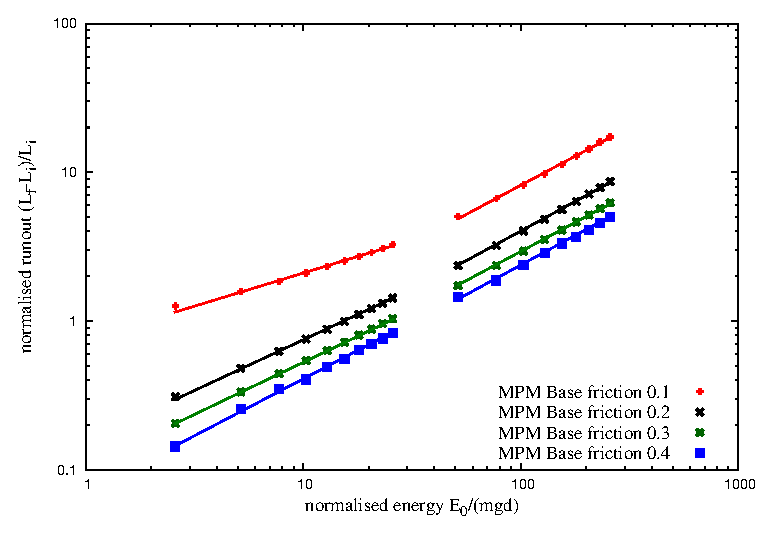
\includegraphics[width=\textwidth]{runout_fric_slope}
\caption{Effect of friction on the run-out distance}
\label{fig:runout_fric_slope}
\end{subfigure}
\\
\begin{subfigure}[b]{0.95\textwidth}
\centering
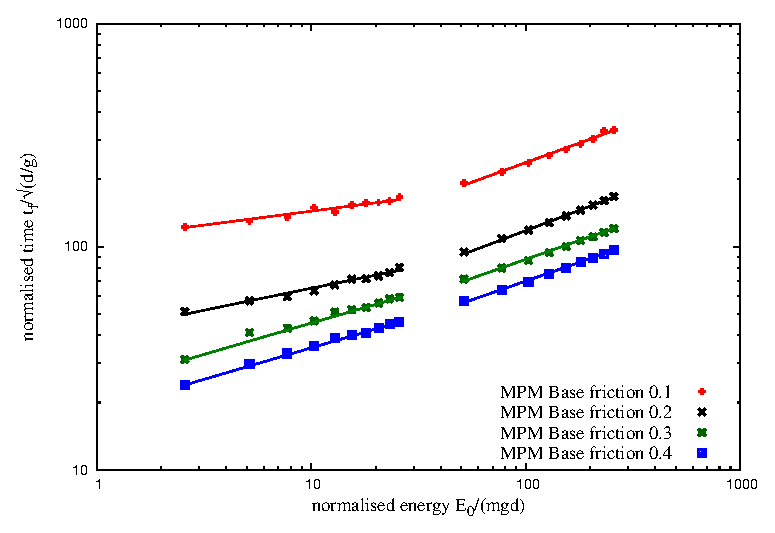
\includegraphics[width=\textwidth]{time_fric_slope}
\caption{Effect of friction on the duration of run-out.}
\label{fig:time_fric_slope}
\end{subfigure}
\caption{Effect of friction on the run-out behaviour}
\label{fig:fric_slope}
\end{figure}

-------------------------------------------------------------------------------

\subsection*{Mode of dissipation}

\begin{figure}[tbph]
\centering
\begin{subfigure}[b]{0.95\textwidth}
\centering
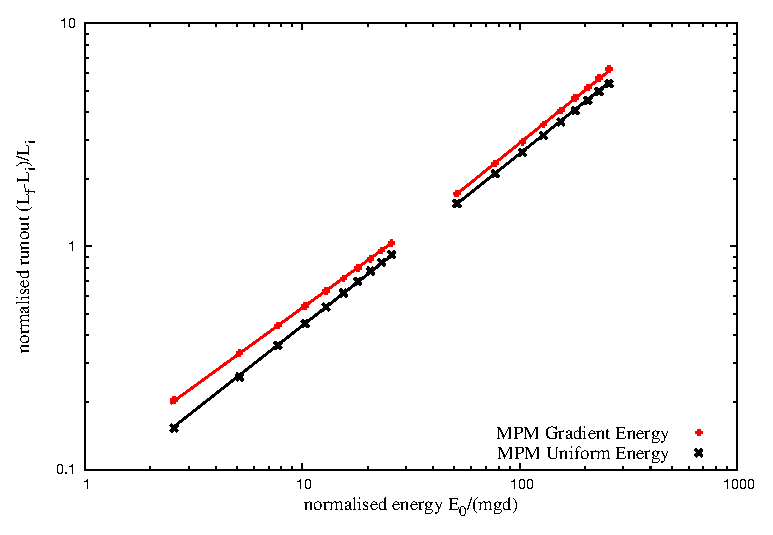
\includegraphics[width=\textwidth]{Runout_Eo_GU}
\caption{Run-out distance as a function of normalised input kinetic energy}
\label{fig:Runout_Eo_GU}
\end{subfigure}
\\
\begin{subfigure}[b]{0.95\textwidth}
\centering
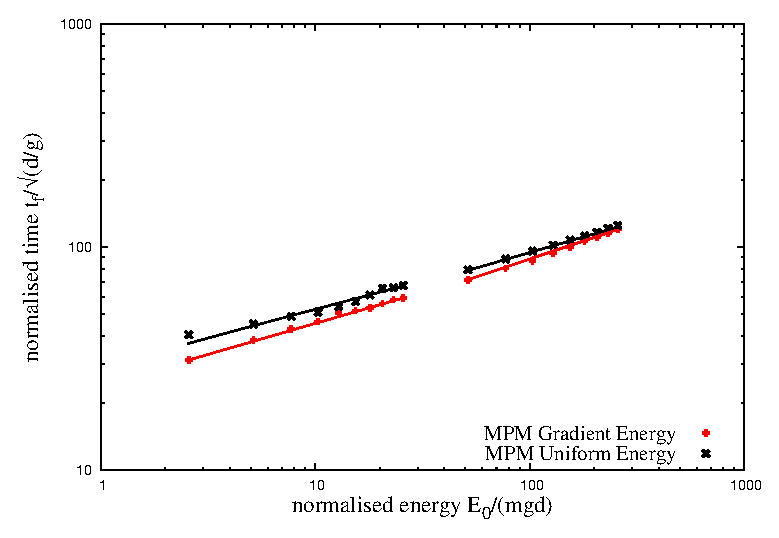
\includegraphics[width=\textwidth]{time_Eo_GU}
\caption{Duration of run-out as a function of normalised input kinetic energy}
\label{fig:time_Eo_GU}
\end{subfigure}
\caption{Effect of input velocity distribution on the run-out behaviour}
\label{fig:GU}
\end{figure}

\begin{figure}[tbph]
\centering
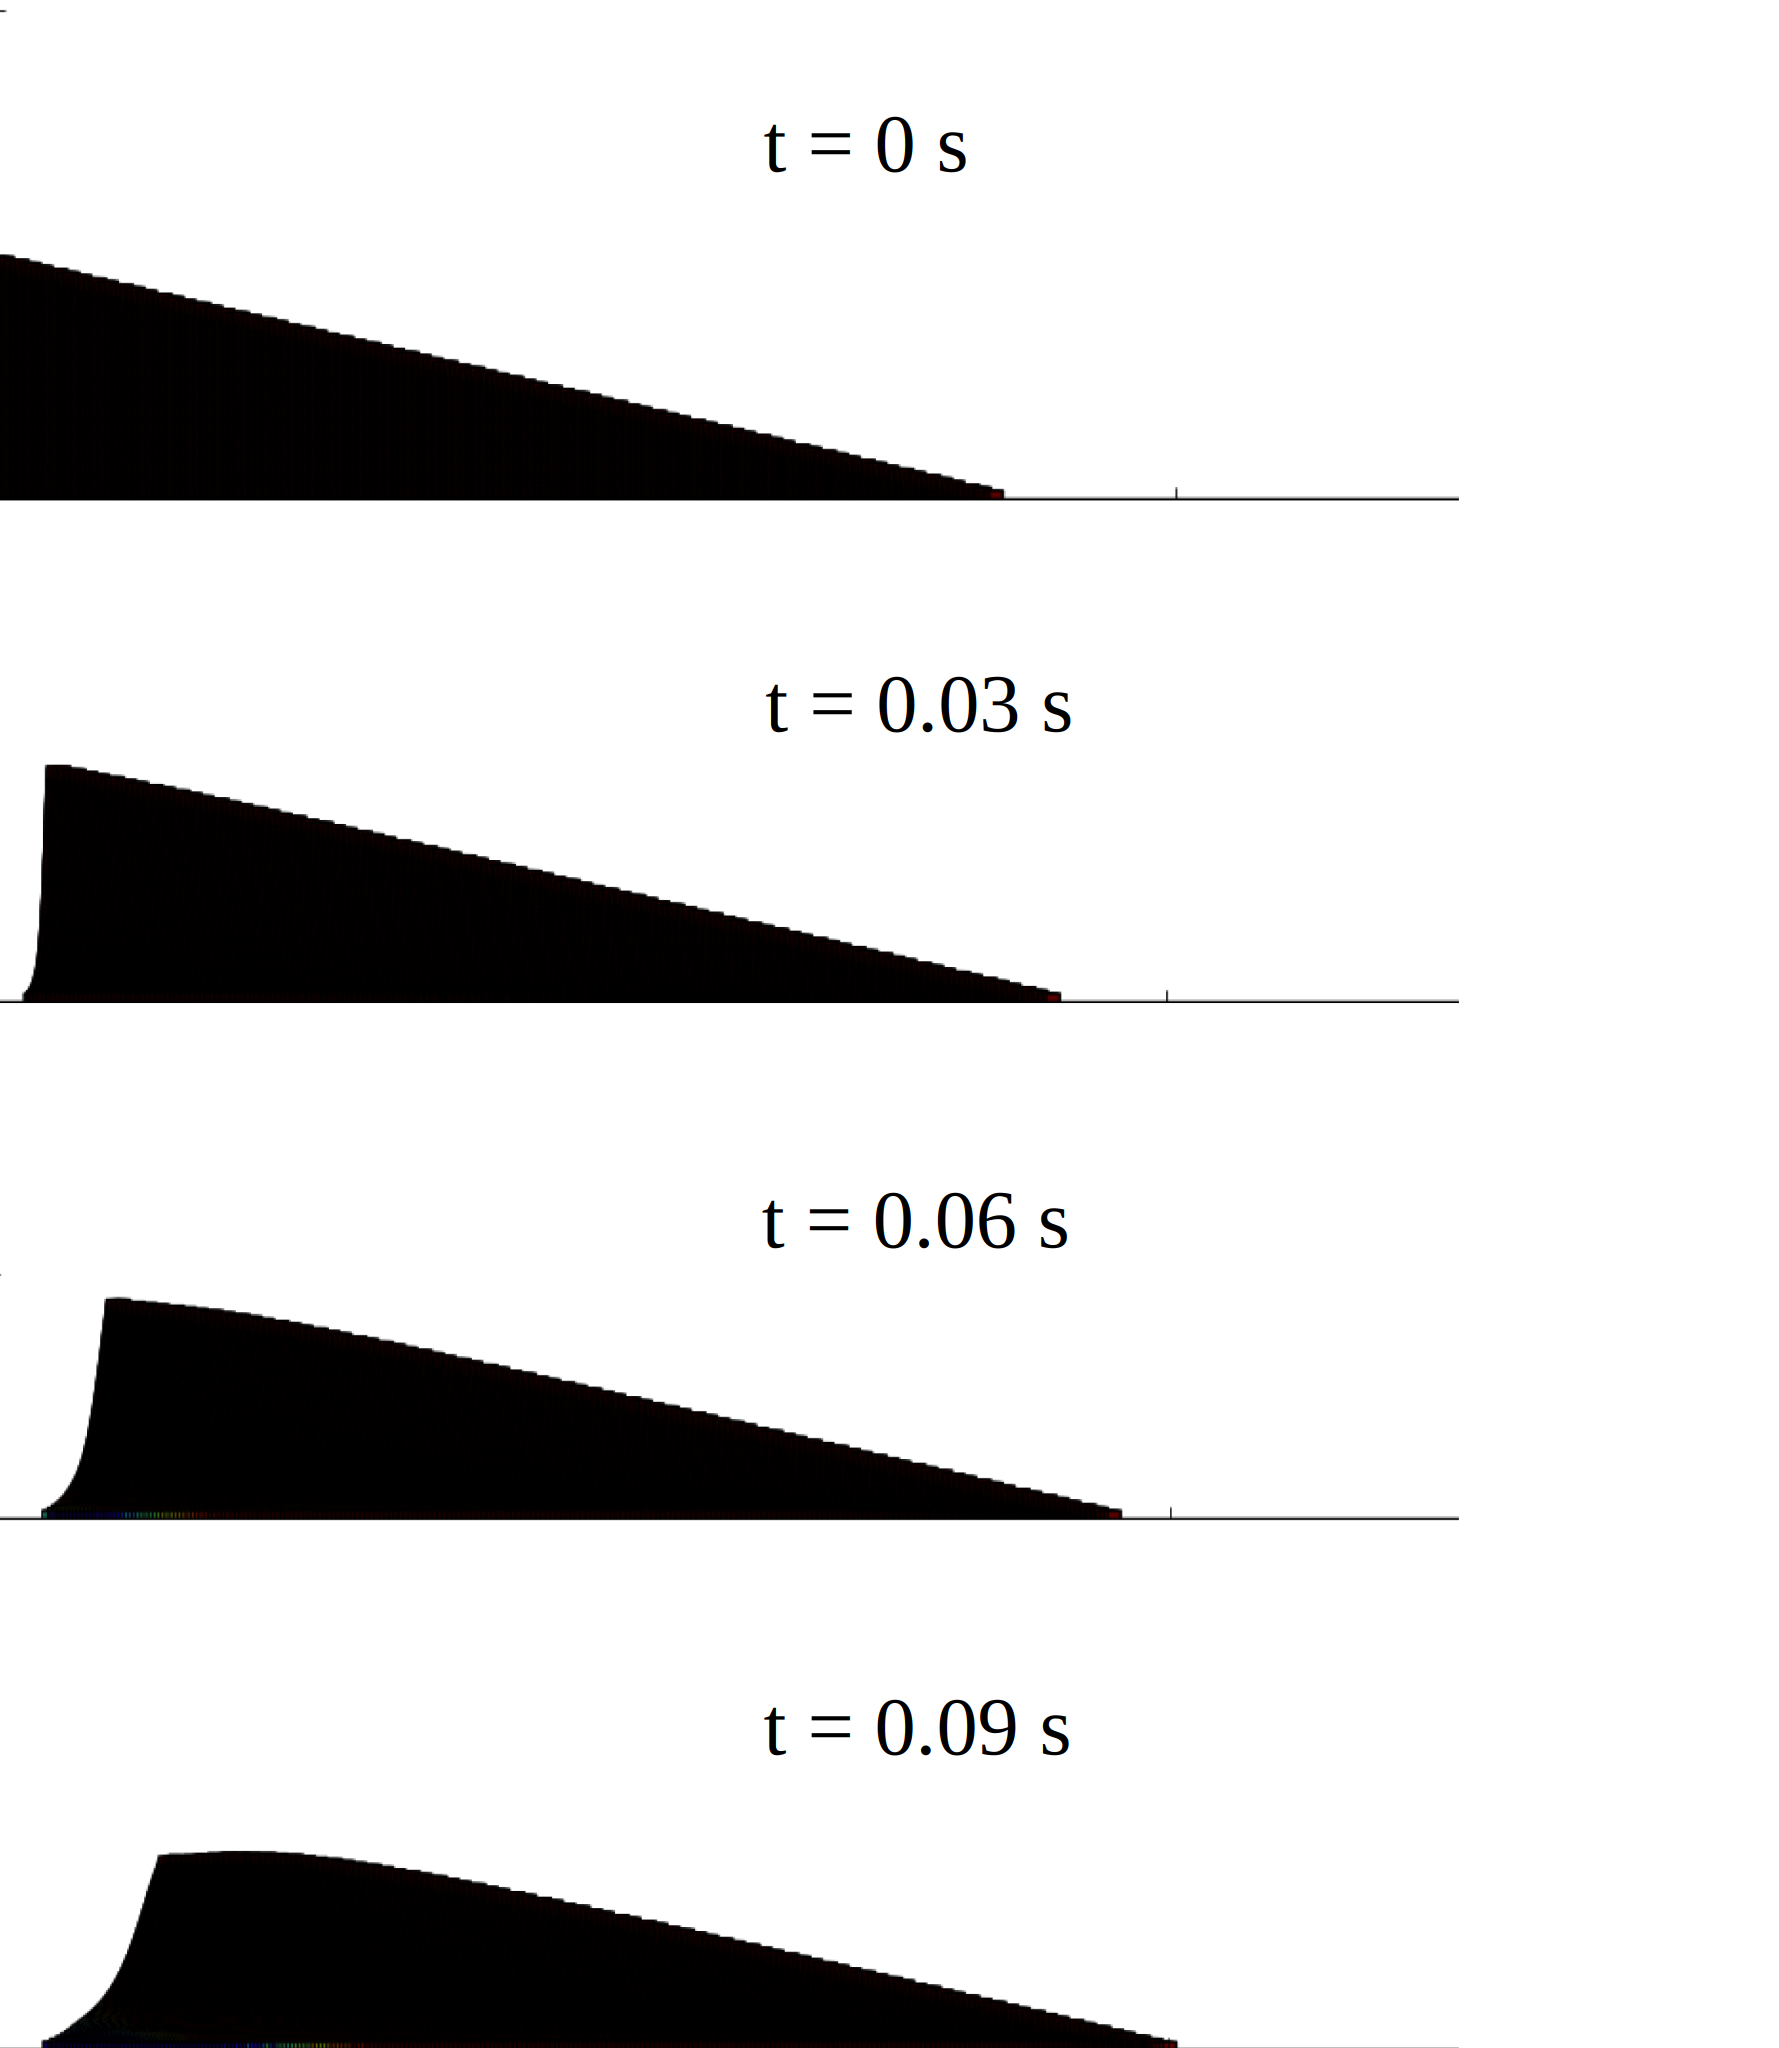
\includegraphics[width=\textwidth]{Uniform_Slope_Profile_200J}
\caption{Snapshots of MPM simulations of the evolution of granular pile 
subjected to a gradient impact energy $E_0 = 61 \ mgd$.}
\label{fig:Uniform_Slope_Profile_200J}
\end{figure}

\begin{figure}[tbph]
\centering
\includegraphics[width=\textwidth]{Uniform_Slope_DEM_200J}
\caption{Snapshots of DEM simulations of the evolution of granular pile 
subjected to a gradient impact energy $E_0 = 61 \ mgd$.}
\label{fig:Uniform_Slope_DEM_200J}
\end{figure}

%-------------------------------------------------------------------------------


The choice of this geometry was motivated by our main goal  to focus on the 
effect of an input energy on the consecutive dynamics of a granular material.
For the range of input energies investigated in this pushing test by means of 
contact dynamics simulations, we observed a power-law dependence of the 
run-out distance and time with non-trivial exponents. This is a central result 
of this work as it reveals that the power-law behaviour is a generic feature of 
granular dynamics. The values of the exponents are not simple functions of 
the geometry. 

We also evidenced two regimes with different values of the exponents: 
a low-energy regime and a high-energy regime. The first regime  
reflects mainly the destabilization of the pile by the quake with a run-out time 
independent of the input energy whereas the second regime is governed by the 
spreading dynamics induced by the higher value of the input energy. We showed 
that the evolution of the pile in this high-energy regime can be described by a 
characteristic decay time and the energy available at the end of the first 
stage where the pile is destabilized by the quake. 

This work may be pursued along two directions: 1) experimental 
realization of a similar setup with different modes of energy injection and 
2) investigating the effect of various particle shapes or the presence of an 
ambient fluid. Although numerical simulations are generally reliable 
with realistic results found in the past studies of steady flows, we believe 
that the transients are more sensitive situations than steady states and the  
experiments are necessary for checking the validation of the results suggested 
by the simulations. Provided a convenient method is used for supplying kinetic 
energy homogeneously into a pile, our configuration is also interesting for 
the investigation of the behavior of a pile immersed in a viscous 
fluid.

\subsection{Effect of material points}
\label{sec:MPM_points_per_cell}
\begin{figure}[tbhp]
\centering
\begin{subfigure}[b]{0.95\textwidth}
\includegraphics[width=\textwidth]{Runout_50}
\caption{$E_0=12.7mgd$}
\label{fig:Runout_50}
\end{subfigure}
\\
\begin{subfigure}[b]{0.95\textwidth}
\centering
\includegraphics[width=\textwidth]{Runout_500}
\caption{$E_0=152mgd$}
\label{fig:Runout_500}
\end{subfigure}
\caption{Evolution of run-out with time for varying material points per cell.}
\label{fig:Runout_MPM}
\end{figure}


\begin{figure}[tbhp]
\centering
\begin{subfigure}[b]{0.95\textwidth}
\includegraphics[width=\textwidth]{KE_50}
\caption{$E_0=12.7mgd$.}
\label{fig:KE_50}
\end{subfigure}
\\
\begin{subfigure}[b]{0.95\textwidth}
\centering
\includegraphics[width=\textwidth]{KE_500}
\caption{$E_0=152mgd$}
\label{fig:KE_500}
\end{subfigure}
\caption{Evolution of kinetic with time for varying material points per cell}
\label{fig:KE_MPM}
\end{figure}

\begin{figure}[tbhp]
\centering
\begin{subfigure}[b]{0.95\textwidth}
\includegraphics[width=\textwidth]{50}
\caption{$E_0=12.7mgd$.}
\label{fig:50}
\end{subfigure}
\\
\begin{subfigure}[b]{0.95\textwidth}
\centering
\includegraphics[width=\textwidth]{500}
\caption{$E_0=152mgd$.}
\label{fig:500}
\end{subfigure}
\caption{Evolution of run-out and duration of flow  for varying material points 
per cell.}
\label{fig:MPM_Size_Effect}
\end{figure}

\subsection{Comparison with granular column collapse}


\begin{figure}[tbhp]
\centering
\includegraphics[width=0.95\textwidth]{Slope_Column}
\caption{Comparison of column collapse with slope subjected to impact loading.}
\label{fig:Slope_Column}
\end{figure}

\section{Summary}
Multi-scale simulation of granular column collapse was performed to understand 
the ability and limitations of continuum models to capture the micro-mechanics 
of dense granular flows. The run-out behaviour predicted by both continuum and 
DEM simulations matches for columns with small aspect ratios, where the 
dissipation is predominantly frictional. However, MPM predicts larger run-out 
distances for columns with higher aspect ratios. Energy evolution studies using 
DEM simulations reveal that the run-out behaviour is independent of frictional 
properties of the granular material and collision predominates the initial 
free-fall regime. The lack of a collisional energy dissipation mechanism in MPM 
results in over prediction of run-out distances. 
